% Options for packages loaded elsewhere
\PassOptionsToPackage{unicode}{hyperref}
\PassOptionsToPackage{hyphens}{url}
%
\documentclass[
  man,floatsintext]{apa6}
\usepackage{amsmath,amssymb}
\usepackage{lmodern}
\usepackage{iftex}
\ifPDFTeX
  \usepackage[T1]{fontenc}
  \usepackage[utf8]{inputenc}
  \usepackage{textcomp} % provide euro and other symbols
\else % if luatex or xetex
  \usepackage{unicode-math}
  \defaultfontfeatures{Scale=MatchLowercase}
  \defaultfontfeatures[\rmfamily]{Ligatures=TeX,Scale=1}
\fi
% Use upquote if available, for straight quotes in verbatim environments
\IfFileExists{upquote.sty}{\usepackage{upquote}}{}
\IfFileExists{microtype.sty}{% use microtype if available
  \usepackage[]{microtype}
  \UseMicrotypeSet[protrusion]{basicmath} % disable protrusion for tt fonts
}{}
\makeatletter
\@ifundefined{KOMAClassName}{% if non-KOMA class
  \IfFileExists{parskip.sty}{%
    \usepackage{parskip}
  }{% else
    \setlength{\parindent}{0pt}
    \setlength{\parskip}{6pt plus 2pt minus 1pt}}
}{% if KOMA class
  \KOMAoptions{parskip=half}}
\makeatother
\usepackage{xcolor}
\usepackage{graphicx}
\makeatletter
\def\maxwidth{\ifdim\Gin@nat@width>\linewidth\linewidth\else\Gin@nat@width\fi}
\def\maxheight{\ifdim\Gin@nat@height>\textheight\textheight\else\Gin@nat@height\fi}
\makeatother
% Scale images if necessary, so that they will not overflow the page
% margins by default, and it is still possible to overwrite the defaults
% using explicit options in \includegraphics[width, height, ...]{}
\setkeys{Gin}{width=\maxwidth,height=\maxheight,keepaspectratio}
% Set default figure placement to htbp
\makeatletter
\def\fps@figure{htbp}
\makeatother
\setlength{\emergencystretch}{3em} % prevent overfull lines
\providecommand{\tightlist}{%
  \setlength{\itemsep}{0pt}\setlength{\parskip}{0pt}}
\setcounter{secnumdepth}{-\maxdimen} % remove section numbering
% Make \paragraph and \subparagraph free-standing
\ifx\paragraph\undefined\else
  \let\oldparagraph\paragraph
  \renewcommand{\paragraph}[1]{\oldparagraph{#1}\mbox{}}
\fi
\ifx\subparagraph\undefined\else
  \let\oldsubparagraph\subparagraph
  \renewcommand{\subparagraph}[1]{\oldsubparagraph{#1}\mbox{}}
\fi
\newlength{\cslhangindent}
\setlength{\cslhangindent}{1.5em}
\newlength{\csllabelwidth}
\setlength{\csllabelwidth}{3em}
\newlength{\cslentryspacingunit} % times entry-spacing
\setlength{\cslentryspacingunit}{\parskip}
\newenvironment{CSLReferences}[2] % #1 hanging-ident, #2 entry spacing
 {% don't indent paragraphs
  \setlength{\parindent}{0pt}
  % turn on hanging indent if param 1 is 1
  \ifodd #1
  \let\oldpar\par
  \def\par{\hangindent=\cslhangindent\oldpar}
  \fi
  % set entry spacing
  \setlength{\parskip}{#2\cslentryspacingunit}
 }%
 {}
\usepackage{calc}
\newcommand{\CSLBlock}[1]{#1\hfill\break}
\newcommand{\CSLLeftMargin}[1]{\parbox[t]{\csllabelwidth}{#1}}
\newcommand{\CSLRightInline}[1]{\parbox[t]{\linewidth - \csllabelwidth}{#1}\break}
\newcommand{\CSLIndent}[1]{\hspace{\cslhangindent}#1}
\ifLuaTeX
\usepackage[bidi=basic]{babel}
\else
\usepackage[bidi=default]{babel}
\fi
\babelprovide[main,import]{english}
% get rid of language-specific shorthands (see #6817):
\let\LanguageShortHands\languageshorthands
\def\languageshorthands#1{}
% Manuscript styling
\usepackage{upgreek}
\captionsetup{font=singlespacing,justification=justified}

% Table formatting
\usepackage{longtable}
\usepackage{lscape}
% \usepackage[counterclockwise]{rotating}   % Landscape page setup for large tables
\usepackage{multirow}		% Table styling
\usepackage{tabularx}		% Control Column width
\usepackage[flushleft]{threeparttable}	% Allows for three part tables with a specified notes section
\usepackage{threeparttablex}            % Lets threeparttable work with longtable

% Create new environments so endfloat can handle them
% \newenvironment{ltable}
%   {\begin{landscape}\begin{center}\begin{threeparttable}}
%   {\end{threeparttable}\end{center}\end{landscape}}
\newenvironment{lltable}{\begin{landscape}\begin{center}\begin{ThreePartTable}}{\end{ThreePartTable}\end{center}\end{landscape}}

% Enables adjusting longtable caption width to table width
% Solution found at http://golatex.de/longtable-mit-caption-so-breit-wie-die-tabelle-t15767.html
\makeatletter
\newcommand\LastLTentrywidth{1em}
\newlength\longtablewidth
\setlength{\longtablewidth}{1in}
\newcommand{\getlongtablewidth}{\begingroup \ifcsname LT@\roman{LT@tables}\endcsname \global\longtablewidth=0pt \renewcommand{\LT@entry}[2]{\global\advance\longtablewidth by ##2\relax\gdef\LastLTentrywidth{##2}}\@nameuse{LT@\roman{LT@tables}} \fi \endgroup}

% \setlength{\parindent}{0.5in}
% \setlength{\parskip}{0pt plus 0pt minus 0pt}

% \usepackage{etoolbox}
\makeatletter
\patchcmd{\HyOrg@maketitle}
  {\section{\normalfont\normalsize\abstractname}}
  {\section*{\normalfont\normalsize\abstractname}}
  {}{\typeout{Failed to patch abstract.}}
\patchcmd{\HyOrg@maketitle}
  {\section{\protect\normalfont{\@title}}}
  {\section*{\protect\normalfont{\@title}}}
  {}{\typeout{Failed to patch title.}}
\makeatother
\shorttitle{Language Input to Blind and Sighted}
\keywords{keywords\newline\indent Word count: X}
\usepackage{lineno}

\linenumbers
\usepackage{csquotes}
\ifLuaTeX
  \usepackage{selnolig}  % disable illegal ligatures
\fi
\IfFileExists{bookmark.sty}{\usepackage{bookmark}}{\usepackage{hyperref}}
\IfFileExists{xurl.sty}{\usepackage{xurl}}{} % add URL line breaks if available
\urlstyle{same} % disable monospaced font for URLs
\hypersetup{
  pdftitle={Comparing Language Input in Homes of Blind and Sighted Children: Insights from Daylong Recordings},
  pdfauthor={Erin Campbell1, Lillianna Righter1, Eugenia Lukin1, \& Elika Bergelson1},
  pdflang={en-EN},
  pdfkeywords={keywords},
  hidelinks,
  pdfcreator={LaTeX via pandoc}}

\title{Comparing Language Input in Homes of Blind and Sighted Children: Insights from Daylong Recordings}
\author{Erin Campbell\textsuperscript{1}, Lillianna Righter\textsuperscript{1}, Eugenia Lukin\textsuperscript{1}, \& Elika Bergelson\textsuperscript{1}}
\date{}


\note{

\textbf{Conflicts of Interest}: The authors have no conflicts of interest to report.
\textbf{Funding}: This work was supported by the National Science Foundation CAREER grant (BCS-1844710) to EB and Graduate Research Fellowship (2019274952) to EC.

}

\affiliation{\vspace{0.5cm}\textsuperscript{1} Department of Psychology \& Neuroscience, Duke University, Durham, NC}

\begin{document}
\maketitle

\hypertarget{abstract}{%
\section{Abstract}\label{abstract}}

\textbf{Purpose:}This study compared language input to young blind children and their sighted peers in naturalistic home settings.

\textbf{Methods:} Using the LENA audio recorder, naturalistic speech in the home was captured and analyzed for various dimensions of language input, including quantitative, interactive, linguistic, and conceptual features.

\textbf{Results:} Our data showed far more similarity than difference across groups, with all differences being small in magnitude. Both groups received similar speech quantity, interactiveness, and lexical diversity. Fine-grained analysis revealed that blind children's language environments contained longer utterances, more temporal displacement, and content words that are harder for children to interact with, suggesting greater similarity to adult-directed speech.

\textbf{Conclusions:} The findings challenge the notion that blind children's language input places them at a disadvantage and suggest that blind children receive rich and complex language input that can support their language development.

\hypertarget{introduction}{%
\section{Introduction}\label{introduction}}

The early language skills of blind children are highly variable (E. E. Campbell, Casillas, \& Bergelson, submitted), with some blind children demonstrating age-appropriate vocabulary from the earliest stages of language learning (Ann Bigelow, 1987; E. E. Campbell et al., submitted; Landau \& Gleitman, 1985), while others experience large and persistent language delays (E. E. Campbell et al., submitted). By adulthood, blind individuals are fluent speakers of their language and are even reported to have faster auditory and lexical processing skills than sighted adults (Röder, Demuth, Streb, \& Rösler, 2003; Röder, Rösler, \& Neville, 2000). The causes of this variability and the later ability to ``catch up'' remain poorly understood: what could make the language learning problem different and initially more difficult for the blind child? There are multiple possible contributors to the variability in language development for blind children, including characteristics of the child (e.g., visual acuity, comorbid conditions, cognitive ability, gender) as well as characteristics of the environment (e.g., access to early intervention services; school setting; caretakers tailoring interactions to their child's sensory access). Here, we compare the language environment of blind children to that of their sighted peers. In doing so, we can begin to untangle the role that perceptual input plays in shaping children's language environment, and better understand the interlocking factors that may contribute to variability in blind children's early language abilities.

\hypertarget{why-would-input-matter}{%
\subsection{Why would input matter?}\label{why-would-input-matter}}

Among both typically-developing children and children with developmental differences, language input can predict variability in language outcomes (Anderson, Graham, Prime, Jenkins, \& Madigan, 2021, 2021; Gilkerson et al., 2018; Huttenlocher, Haight, Bryk, Seltzer, \& Lyons, 1991; Huttenlocher, Waterfall, Vasilyeva, Vevea, \& Hedges, 2010; Rowe, 2008, 2012). There are many ways to operationalize language input, that tend to be grouped into \textbf{quantity of language input} and \textbf{input characteristics} (MacLeod \& Demers, 2023). Quantity of language input can be broadly construed as the number of words or utterances a child is exposed to. At a coarse level, children who are exposed to more speech (or sign, Watkins, Pittman, \& Walden, 1998) tend to have better language outcomes (Anderson et al., 2021; Gilkerson et al., 2018; Huttenlocher et al., 1991; Rowe, 2008). However, if only the \emph{amount} of language exposure mattered, then infants should be able to sit in front of the television all day and become fluent language users. Yet young children struggle to learn language from just from exposure to large quantities of speech (e.g., Roseberry, Hirsh-Pasek, \& Golinkoff, 2014 May-Jun), so something about the \emph{type} of language input must matter.

The specific characteristics of that language input are perhaps even more influential (Hirsh-Pasek et al., 2015; Rowe, 2012), although it is somewhat trickier to turn the qualitative characteristics of language input into operationalizable properties. Rowe and Snow (Rowe \& Snow, 2020) divide this space into three dimensions of language input: interactive features (e.g., parent responsiveness, speech directed \emph{to} child vs.~overheard; conversational turn-taking), linguistic features (e.g., lexical diversity, grammatical complexity), and conceptual features (e.g., topic diversity).

Parents' active response to their children's actions and utterances supports their learning. Prior literature reports that back-and-forth communicative exchanges (also known as conversational turns) between caregivers and children predict better language outcomes across infancy (Donnellan, Bannard, McGillion, Slocombe, \& Matthews, 2020; Goldstein \& Schwade, 2008) and toddlerhood (Hirsh-Pasek et al., 2015; Romeo et al., 2018). Another way to quantify the extent to which caregivers and infants interact during language input is by looking at how much speech is directed \emph{to} the child (as opposed to, for example, an overheard conversation between adults). The amount of child-directed speech in children's input {[}at least in Western contexts; Casillas, Brown, and Levinson (2020){]} is associated with children's vocabulary and lexical processing (Rowe, 2008; Shneidman, Arroyo, Levine, \& Goldin-Meadow, 2013; Weisleder \& Fernald, 2013) Parents' interaction with their child and the world around them ties together the linguistic and conceptual characteristics of the language input, to which we turn next.

The linguistic characteristics of language input can be thought of in terms of which words are used and how those words are combined, both of which have measurable associations with children's language growth. Two commonly-analyzed linguistic features are lexical diversity {[}often measured as type/token ratio; CITE{]} and syntactic complexity {[}often measured by mean length of utterance, CITE{]}. Sighted toddlers who are exposed to greater diversity of words in their language input are reported to have larger vocabulary scores (Anderson et al., 2021; Hsu, Hadley, \& Rispoli, 2017; Huttenlocher et al., 2010; Rowe, 2012; Weizman \& Snow, 2001). Likewise, the diversity and complexity of syntactic constructions in parental language input is associated both with children's vocabulary growth and structure diversity in their own productions (De Villiers, 1985; Hadley et al., 2017; Hoff, 2003 Sep-Oct; Huttenlocher, Vasilyeva, Cymerman, \& Levine, 2002; Huttenlocher et al., 2010; Naigles \& Hoff-Ginsberg, 1998).

The conceptual dimension of language input aims to capture the extent to which the language signal maps onto objects and events in the world (Rowe \& Snow, 2020). The conceptual aspects that are most informative may shift across developmental time: as children develop, their ability to represent abstract, displaced, decontextualized referents improves (Bergelson \& Swingley, 2013; Kramer, Hill, \& Cohen, 1975; Luchkina, Xu, Sobel, \& Morgan, 2020). For example, infants are more likely to learn a new word when the referent is perceptually salient, dominating their field of view (Yu \& Smith, 2012; Yurovsky, Smith, \& Yu, 2013). Parents responding to a child's point and labeling the object of interest might boost learning in that instance (Lucca \& Wilbourn, 2018). By contrast, \emph{displaced} language use-- that is, talking about past, future, or hypothetical events, or people and items that are not currently present in the environment-- may be beneficial at later stages of development (Rowe, 2013). Indeed, greater decontextualized language use in speech to toddlers predicts aspects of children's own language in kindergarten and beyond (Demir, Rowe, Heller, Goldin-Meadow, \& Levine, 2015; Rowe, 2012; Uccelli, Demir-Lira, Rowe, Levine, \& Goldin-Meadow, 2019).

From this review, it appears that sighted children learn about the world and language simultaneously from many sources, including sensory perception, linguistic input, and conceptual and social knowledge. For blind children, however, language input may constitute a greater proportion of the available clues for learning than for sighted children; in the absence of visual input, language is an important source of information about the world (E. E. Campbell \& Bergelson, 2022). Syntactic structure in particular provides cues to word meaning that may be lost without visual cues, such as the relationship between two entities that aren't within reach (Gleitman, 1990).So far, we have presented a pattern wherein the features of the input that are most helpful for language learning change over the course of children's development: early on, many of these cues require visual access, such as parental gaze, shared visual attention, pointing to remote object and the presence of salient objects in the visual field. Later in development the handholds to language learning become more abstract, but more equitably accessible to blind and sighted children: more sophisticated language knowledge is built from information in the language signal and the child's prior knowledge, neither of which require visual interfacing. This may be part of the reason why language delays are common in blind toddlers, but often resolved in older childhood (Landau \& Gleitman, 1985). If direct sensory access to referents provides an initial ``brute force'' mechanism for mapping words onto meanings, it may take longer for blind children to acquire the first few words. By hypothesis, once this initial seed of lexical knowledge is acquired, blind children and sighted children alike are able to use more abstract and linguistic features as cues, and learning can proceed more rapidly thereafter (Babineau, de Carvalho, Trueswell, \& Christophe, 2021; Babineau, Havron, Dautriche, de Carvalho, \& Christophe, 2022; E. E. Campbell \& Bergelson, 2022). Nevertheless, we cannot assume that access to visual experience is the \emph{only} difference in the language learning experiences for blind and sighted children; the language input itself may differ for blind children relative to sighted children.

\hypertarget{why-would-the-input-differ}{%
\subsection{Why would the input differ?}\label{why-would-the-input-differ}}

Speakers regularly tailor input to communicate efficiently with the listener (Grice, 1975). Parents are sensitive to their child's developmental level and tune language input accordingly (Snow, 1972; Vygotsky \& Cole, 1978). Child-directed speech is one example--whereby parents speak to young children with exaggerated prosody, slower speech rate, and increased vowel clarity (Bernstein Ratner, 1984; Fernald, 1989), which is in some cases helpful to the young language learner (Thiessen, Hill, \& Saffran, 2005). When interacting with infants and toddlers, parents repeat words more often than when interacting with older children or adults (Snow, 1972). Communicative tailoring is also common in language input to children with disabilities, who tend to receive simplified, more directive language input, and less interactive input compared to typically-developing children (Dirks, Stevens, Kok, Frijns, \& Rieffe, 2020; Yoshinaga-Itano, Sedey, Mason, Wiggin, \& Chung, 2020).

In addition to tailoring communication to children's developmental level, speakers also adjust their conversation in accordance with the conversation partner's sensory access (Gergle, Kraut, \& Fussell, 2004; Grigoroglou, Edu, \& Papafragou, 2016). In a noisy environment, speakers will adapt the acoustic-phonetic features of their speech with the intent to make it easier for their interlocutor to understand them (Hazan \& Baker, 2011), which demonstrates sensitivity to even temporary sensory conditions of their conversation partner. When describing scenes, speakers aim to provide the information their listeners lack but avoid redundant visual description (Grice, 1975; Ostarek, Paridon, \& Montero-Melis, 2019). During in-lab tasks with sighted participants, participants tailor their descriptions and requests by verbally providing visually-absent cues when an object is occluded to their partner (Hawkins, Gweon, \& Goodman, 2021; Jara-Ettinger \& Rubio-Fernandez, 2021; Rubio-Fernandez, 2019). These results suggest that adults and even infants (Chiesa, Galati, \& Schmidt, 2015; N. Ganea et al., 2018; Senju et al., 2013) can flexibly adapt communication to the visual and auditory abilities of their partner.

Taking these results into account, we might expect parents to verbally compensate for missing visual input, perhaps providing more description of the child's environment. Prior research doesn't yield a clear answer. Several early studies suggest differences in the concepts parents discuss: caregivers of blind children restrict conversation to things that the blind child is currently engaged with, rather than attempt to redirect their attention to other stimuli (Andersen, Dunlea, \& Kekelis, 1993; J. Campbell, 2003; Kekelis \& Andersen, 1984; though c.f., Moore \& McConachie, 1994). Studies of input to blind children in naturalistic settings report that parents use \emph{fewer} declaratives and \emph{more} imperatives than parents of sighted children, suggesting that blind children might be receiving less description than sighted children (Kekelis \& Andersen, 1984; Landau \& Gleitman, 1985). Other studies report that parents adapt their interactions to their children's visual abilities, albeit in specific contexts. Tadić, Pring, and Dale (2013 Nov-Dec) and colleagues find that in a structured book reading task, parents of blind children provide more descriptive utterances than parents of sighted children. Further, parents of blind children provide more tactile cues to initiate interactions or establish joint attention (Preisler, 1991; Urwin, 1983, 1984), which may serve the same social role as shared gaze in sighted children. These mixed results suggest that parents of blind children might alter language input in some domains but not others. The apparent conflict in results may be exacerbated by the difficulty of recruiting specialized populations to participate in research: the small (in most cases single-digit) sample sizes of prior work limits our ability to generalize about any principled differences in the input to blind infants.

\hypertarget{the-present-study}{%
\subsection{The Present Study}\label{the-present-study}}

Reaching a better understanding of how sensory perception and linguistic input interact to influence blind children's language outcomes is of great scientific, clinical, and educational importance. If properties of language input influence the likelihood of language delays among blind infants and toddlers (E. E. Campbell et al., submitted), capturing this variation may reveal a more nuanced picture of how infants use the input to learn language. In the present study, we examine daylong recordings of the naturalistic language environments of blind and sighted children in order to characterize the input to each group. Using both automated measures and manual transcription of these recordings, we measure input quantity (adult word count) and analyze several characteristics that have been previously suggested to be information-rich learning cues, including interactivity (conversational turn counts, proportion of child-directed speech), conceptual features (temporal displacement, sensory modality), and linguistic complexity (type/token ratio and mean length of utterance).

\hypertarget{methods}{%
\section{Methods}\label{methods}}

\hypertarget{participants}{%
\subsection{Participants}\label{participants}}

15 blind infants and their families participated in this study. Blind participants were recruited through ophthalmologist referral, preschools, early intervention programs, social media, and word of mouth. To be eligible for this study, participants had to be 6--30 months old, have no additional disabilities (developmental delays; intellectual disabilities, or hearing loss), and be exposed to \(\geq\) 75\% English at home. To control for the wide age range of the study, each blind participant was matched to a sighted participant, based on age (\(\pm\) 6 weeks), gender, maternal education (\(\pm\) one education level: less than high school diploma, high school diploma, some college / Associate's, Bachelor's, graduate school), and number of siblings (\(\pm\) 1 sibling). We prioritized matching each characteristic as closely as possible in the preceding order. Caregivers were asked to complete a demographics survey and the MacArthur-Bates Communicative Development Inventory (CDI, Fenson et al., 1994) within one week of the home language recording. See Table \ref{tab:participant-characteristics} for sample characteristics.

\begin{table}[ht]
\centering
\begin{tabular}{lrrr}
  \hline
Variable & Blind & Sighted & Overall \\ 
  \hline
\vspace*{0.1cm} \\ \textbf{Age in months      } &  &  &  \\ 
  \hskip .5cm    Mean (SD) & 15.77 (8.20) & 16.15 (8.15) & 15.96 (8.04) \\ 
  \hskip .5cm    Min, Max & 6.41, 30.38 & 6.18, 31.76 & 6.18, 31.76 \\ 
  \hskip .5cm \textbf{ } &   &   &   \\ 
  \vspace*{0.1cm} \\ \textbf{Gender      } &  &  &  \\ 
  \hskip .5cm   (Col \%) &  &  &  \\ 
  \hskip .5cm \textbf{  F} & 7 (43.75\%) & 7 (43.75\%) & 14 (43.75\%) \\ 
  \hskip .5cm \textbf{  M} & 9 (56.25\%) & 9 (56.25\%) & 18 (56.25\%) \\ 
  \hskip .5cm \textbf{ } &   &   &   \\ 
  \vspace*{0.1cm} \\ \textbf{Maternal education level      } &  &  &  \\ 
  \hskip .5cm   (Col \%) &  &  &  \\ 
  \hskip .5cm \textbf{  Some college} & 0 ( 0.00\%) & 0 ( 0.00\%) & 0 ( 0.00\%) \\ 
  \hskip .5cm \textbf{  Associate's degree} & 3 (23.08\%) & 1 ( 7.69\%) & 4 (15.38\%) \\ 
  \hskip .5cm \textbf{  Bachelor's degree} & 1 ( 7.69\%) & 2 (15.38\%) & 3 (11.54\%) \\ 
  \hskip .5cm \textbf{  Master's degree} & 5 (38.46\%) & 9 (69.23\%) & 14 (53.85\%) \\ 
  \hskip .5cm   Missing & 4 (30.77\%) & 1 ( 7.69\%) & 5 (19.23\%) \\ 
  \vspace*{0.1cm} \\ \textbf{Maternal education level      } & 0 ( 0.00\%) & 0 ( 0.00\%) & 0 ( 0.00\%) \\ 
  \hskip .5cm \textbf{ } &   &   &   \\ 
  \vspace*{0.1cm} \\ \textbf{Number of older siblings      } &  &  &  \\ 
  \hskip .5cm    Mean (SD) & 0.50 (0.82) & 1.09 (1.04) & 0.74 (0.94) \\ 
  \hskip .5cm    Min, Max & 0.00, 2.00 & 0.00, 3.00 & 0.00, 3.00 \\ 
  \hskip .5cm \textbf{ } &   &   &   \\ 
  \vspace*{0.1cm} \\ \textbf{Vision diagnosis      } &  &  &  \\ 
  \hskip .5cm   (Col \%) &  &  &  \\ 
  \hskip .5cm \textbf{  Cataracts} & 3 (18.75\%) & - & 3 (18.75\%) \\ 
  \hskip .5cm \textbf{  Leber's Congenital Amaurosis } & 1 ( 6.25\%) & - & 1 ( 6.25\%) \\ 
  \hskip .5cm \textbf{  Microphthalmia } & 2 (12.50\%) & - & 2 (12.50\%) \\ 
  \hskip .5cm \textbf{  Multiple} & 2 (12.50\%) & - & 2 (12.50\%) \\ 
  \hskip .5cm \textbf{  Not specified} & 2 (12.50\%) & - & 2 (12.50\%) \\ 
  \hskip .5cm \textbf{  Ocular albinism} & 2 (12.50\%) & - & 2 (12.50\%) \\ 
  \hskip .5cm \textbf{  Optic Nerve Hypoplasia} & 2 (12.50\%) & - & 2 (12.50\%) \\ 
  \hskip .5cm \textbf{  Retinal Detachments} & 1 ( 6.25\%) & - & 1 ( 6.25\%) \\ 
  \hskip .5cm \textbf{  Retinopathy of Prematurity} & 1 ( 6.25\%) & - & 1 ( 6.25\%) \\ 
  \hskip .5cm \textbf{ } &   &   &   \\ 
  \vspace*{0.1cm} \\ \textbf{Race      } &  &  &  \\ 
  \hskip .5cm   (Col \%) &  &  &  \\ 
  \hskip .5cm \textbf{  American Indian or Alaska Native} & 1 ( 6.25\%) & 0 ( 0.00\%) & 1 ( 3.12\%) \\ 
  \hskip .5cm \textbf{  Black or African American} & 1 ( 6.25\%) & 1 ( 6.25\%) & 2 ( 6.25\%) \\ 
  \hskip .5cm \textbf{  Mixed} & 3 (18.75\%) & 1 ( 6.25\%) & 4 (12.50\%) \\ 
  \hskip .5cm \textbf{  unknown} & 0 ( 0.00\%) & 7 (43.75\%) & 7 (21.88\%) \\ 
  \hskip .5cm \textbf{  White} & 11 (68.75\%) & 7 (43.75\%) & 18 (56.25\%) \\ 
  \hskip .5cm \textbf{ } &   &   &   \\ 
  \vspace*{0.1cm} \\ \textbf{Ethnicity      } &  &  &  \\ 
  \hskip .5cm   (Col \%) &  &  &  \\ 
  \hskip .5cm \textbf{  Hispanic or Latino} & 3 (18.75\%) & 0 ( 0.00\%) & 3 ( 9.38\%) \\ 
  \hskip .5cm \textbf{  Not Hispanic or Latino} & 13 (81.25\%) & 8 (50.00\%) & 21 (65.62\%) \\ 
  \hskip .5cm \textbf{  unknown} & 0 ( 0.00\%) & 8 (50.00\%) & 8 (25.00\%) \\ 
  \hskip .5cm \textbf{ } &   &   &   \\ 
   \hline
\end{tabular}
\end{table}

\hypertarget{recording-procedure}{%
\subsection{Recording Procedure}\label{recording-procedure}}

For the recording portion of the study, caregivers of participating infants received a LENA wearable audio recorder and vest (Ganek \& Eriks-Brophy, 2016; Gilkerson \& Richards, 2008). They were instructed to place the recorder in the vest on the day of their scheduled recording and put the vest on their child from the time they woke up until the recorder automatically shut off after 16 hours (setting the vest nearby during baths, naps, and car rides). They were also informed how to pause the recording at any time, but asked to keep these pauses to a minimum. Actual recording length ranged from 8 hours 17 minutes to 15 hours 59 minutes (Mean: 15 hours 16 minutes).

\hypertarget{processing}{%
\subsection{Processing}\label{processing}}

The audio recordings were first processed by LENA proprietary software, creating algorithmic measures such as conversational turn counts and adult word count. Each recording was then run through an in-house automated sampler that selected 15- non-overlapping 5-minute segments, randomly distributed across the duration of the recording. The process outputs a codeable ELAN file (.eaf, Brugman \& Russel, 2009). Each segment consists of 2 core minutes of annotated time, with 2 minutes of listenable context preceding the annotation clip and 1 minute of additional context following the annotation clip. Each file therefore contains 30 minutes of coded recording time and 75 minutes of total time listened. Because these segments were sampled randomly, and not on a high-volubility measure such as conversational turns or adult speech density, the amount of time with codeable speech input varied for each recording. Indeed, across participants roughly 0\% of the random 2-minute coding segments contained no speech at all. For questions of \emph{how much does a phenomenon occur}, random sampling schemes can help avoid overestimating speech in the input, but for questions of input \emph{content}, randomly selected samples may be too sparse (Pisani, Gautheron, \& Cristia, 2021).

Therefore, we also chose to annotate 5 additional segments specifically for their high density of speech. To select these segments of dense talk, we first conducted an automated analysis of the audio file using the voice type classifier for child-centered daylong recordings (Lavechin, Bousbib, Bredin, Dupoux, \& Cristia, 2021) which identified all human speech in the recording. The entire recording was then broken into 2-minute chunks marked out at zero-second timestamps (e.g.~00:02:00.000 to 00:04:00.000). Each of these chunks was ranked highest to lowest by the total duration of speech contained within the boundaries. For our high volubility sample, we chose the highest-ranked 5 segments of each recording, excluding those that overlapped with already-coded random segments. These high volubility segments allowed us first to characterize features of the language as proportions of the linguistic input children receive, and second, to more closely compare our findings to studies classifying the input during structured play sessions, which paint a denser and differently-proportioned makeup of the language input (Bergelson, Amatuni, Dailey, Koorathota, \& Tor, 2019). In sum, 30 minutes of randomly sampled input and 10 minutes of high-volubility input produced 40 minutes of annotated recording time per child.

\hypertarget{annotation}{%
\subsection{Annotation}\label{annotation}}

Trained annotators listened through each 2-minute segment plus its surrounding context and coded it using the Analyzing Child Language Experiences around the World (ACLEW) Daylong Audio Recording of Children's Linguistic Environments (DARCLE) annotation scheme (Soderstrom et al., 2021). Prior to annotating lab data, annotators are trained on previously coded samples of child recordings and are required to reach 95\% overall agreement with the gold standard version of the file for three different age ranges: 0-7 months, 8-18 months, and 19-36 months. For more information about this annotation scheme and the larger project, please see the \href{https://sites.google.com/view/aclewdid/home}{ACLEW homepage}. Following the first pass, all files were reviewed by a highly-trained ``superchecker'' to ensure the consistency of annotations.

This annotation scheme is designed to capture both utterances by the target child and speech in the child's environment, including adults, other children, and pre-recorded electronic speech (e.g.~toys, television, the radio). Annotators segment the duration of each utterance on a separate coding tier for each unique speaker. Speech by people other than the target child is transcribed using an adapted version of the CHAT transcription style (MacWhinney, 2019; Soderstrom et al., 2021). Because the majority of target children in the project are pre-lexical, utterances produced by the target child are not yet transcribed. Environmental speech is then classified based on the addressee of each utterance: speech directed to a child; adult-directed speech; speech directed to both an adult and a child; speech directed to pets or other animals; speech with an unclear addressee; or speech directed towards a recipient that doesn't fit into another category (e.g., voice control of Siri or Alexa, prayer to a metaphysical entity).

\hypertarget{extracting-measures-of-language-input}{%
\subsection{Extracting Measures of Language Input}\label{extracting-measures-of-language-input}}

To go from our dimensions of interest (quantity, interactiveness, linguistic, conceptual), to quantifiable properties, we used a combination of automated measures {[}generated by the proprietary LENA algorithm; Xu, Yapanel, and Gray (2009){]} and manual measures (generated from the transcriptions made by our trained annotators). These manual annotations can be analyzed for the random segments, the high-volume segments, or both. The decision of which segments to analyze was made according to the goal of the analysis: quantity and interactiveness analyses were conducted on the random samples only, to capture a more representative estimate. Linguistic and conceptual analyses were conducted on all available annotations in order to maximize the amount of speech over which we could calculate them. These measures are summarized in Table \ref{tab:variables-table}.

\begin{table}

\caption{\label{tab:variables-table}Language input variables extracted from recordings.}
\centering
\fontsize{9}{11}\selectfont
\begin{tabular}[t]{>{\raggedright\arraybackslash}p{1.4in}|>{\centering\arraybackslash}p{.8in}|>{\centering\arraybackslash}p{.75in}|>{\raggedright\arraybackslash}p{2.8in}}
\hline
Variable & Coding & Portion of Recording & Description\\
\hline
Adult Word Count / half hour (AWC) & Automated & Whole day & Estimated number of words in recording categorized as nearby adult speech by LENA algorithm\\
\hline
Manual Word Count (WC) & Manual & Random & Number of word tokens from speakers other than target child\\
\hline
Conversational Turn Count / half hour (CTC) & Automated & Whole day & Count of temporally close switches between adult and target-child vocalizations, divided by recording length\\
\hline
Proportion of Child-Directed Speech (Prop. CDS) & Manual & Random & Number of utterances tagged with child addressee out of total number of utterances, from speakers other than target child\\
\hline
Type-Token Ratio & Manual & Random + High Volume & Average of the type-token ratios (number of unique words divided by number of total words) for each of the 100-word bins in their sample\\
\hline
Mean Length of Utterance & Manual + NLP parsing & Random + High Volume & Average number of morphemes per utterance\\
\hline
Proportion of Temporally Displaced Verbs (Prop. Displaced) & Manual + NLP tagging & Random + High Volume & Proportion of verbs that refer to past, future, or hypothetical events\\
\hline
Child-Body-Object Interaction Ratings (CBOI) & Manual + NLP tagging & Random + High Volume & Distribution of ratings of “how much a child can interact with” each word (adjectives, adverbs, nouns, verbs)\\
\hline
Proportion of Highly Visual Words & Manual & Random + High Volume & Proportion of words in the input with high visual association ratings and low ratings for other perceptual modalities\\
\hline
\end{tabular}
\end{table}

\hypertarget{quantity}{%
\subsubsection{Quantity}\label{quantity}}

\hypertarget{adult-word-count}{%
\paragraph{Adult Word Count}\label{adult-word-count}}

To derive this count, first the LENA algorithm segments the recording into clips of varying length. These segments are then classified as female adult speech, male adult speech, target child, other child, overlapping vocalization/noise, electronic noise, noise, silence, or uncertain, each of which is further categorized into ``near'' or ``far''. Only segments that are classified as nearby male or female adult speech are included in the Adult Word Count estimation; Segments that the LENA algorithm identifies as ``far'', ``child'', or ``overlapping'', do not contribute to this count (Xu et al., 2009). Validation work suggests that this automated count correlates strongly with word counts derived from manual annotations (r = .71 -- .92, Lehet, Arjmandi, Houston, \& Dilley, 2021), but Lehet et al. (2021) and colleagues find that the amount of error may vary substantially across families. Compared to short samples that they had manually transcribed and counted, LENA's AWC estimate ranged from undercounting words by 17\% to overcounting words by 208\% (Lehet et al., 2021). Perhaps reassuringly however, meta-analytic work finds that AWC is associated with children's language outcomes across developmental contexts (e.g., autism, hearing loss, Wang, Williams, Dilley, \& Houston, 2020). Because the recordings varied in length ( 8 hours 17 minutes to 15 hours 59 minutes), we normalized AWC by dividing by recording length \footnote{To make this comparable to the manual word count estimates, which are derived from the 30 minutes of randomly sampled annotation, we calculate AWC per half hour.}.

\hypertarget{manual-word-count}{%
\paragraph{Manual Word Count}\label{manual-word-count}}

We also compare a manual count of speech in the children's environment. Manual word count is simply the number of intelligible words in our transcriptions of each child's recording. Speech that was too far or muffled to be intelligible, as well as speech from the target child and electronic speech (TV, radio, toys) are excluded from this count. To try to get a representative estimate of the amount of talk in a children's environment, we use the random samples only for this measure.

By using Adult Word Count and Manual Word Count, we hope to capture complementary estimates of the amount of speech children are exposed to. AWC is less accurate, but commonly used, and provides an estimate of the speech across the whole day. MWC, because it comes from human annotations, is the gold-standard for accurate speech estimates, but is only derived from 30 minutes of the recording.

\hypertarget{interactivity}{%
\subsubsection{Interactivity}\label{interactivity}}

\hypertarget{conversational-turn-count}{%
\paragraph{Conversational Turn Count}\label{conversational-turn-count}}

One commonly used and easily-extracted metric of communicative interaction (e.g., Ganek \& Eriks-Brophy, 2018; Magimairaj, Nagaraj, Caballero, Munoz, \& White, 2022) is conversational turn count (or CTC), an automated measure generated by LENA (Xu et al., 2009). Like AWC, a recent meta-analysis finds that CTC is associated with children's language outcomes (Wang et al., 2020). After tagging vocalizations for speaker identity, LENA algorithm looks for alternations between adult and target child speech in close temporal proximity. The algorithm counts any temporally close (within 5 seconds) switch between adult and target child vocalizations, which can erroneously include non-contingent interactions (e.g., mom talking to dad while the infant babbles to herself nearby), and therefore inflate the count especially for younger ages and in houses with multiple children (Ferjan Ramírez, Hippe, \& Kuhl, 2021). Still, this measure correlates moderately well with manually-coded conversational turns (Busch, Sangen, Vanpoucke, \& van Wieringen, 2018; Ganek \& Eriks-Brophy, 2018), and because participants in our sample are matched on both age and number of siblings, CTC overestimation should not be biased towards either groups. Conversational turn count is calculated over the entire recording, but to normalize for recording length, we divided this by recording length.

\hypertarget{proportion-of-child-directed-speech}{%
\paragraph{Proportion of Child-Directed Speech}\label{proportion-of-child-directed-speech}}

Our other measure of interactivity is the proportion of utterances that are child-directed, derived from the manual annotations. Each proportion was calculated as the number of utterances (produced by someone \emph{other} than the target child) tagged with a child addressee out of the total number of utterances. To try to get a representative measure of child-directed speech in the environment overall (Cychosz, Villanueva, \& Weisleder, 2021), we use the random samples only for this calculation.

\hypertarget{linguistic-features}{%
\subsubsection{Linguistic Features}\label{linguistic-features}}

\hypertarget{type-token-ratio}{%
\paragraph{Type-Token Ratio}\label{type-token-ratio}}

As in previous work (Montag, Jones, \& Smith, 2018; Pancsofar \& Vernon-Feagans, 2006; e.g., Templin, 1957), we calculated the lexical diversity of the input by dividing the number of unique words by the total number of words (i.e., the type-token ratio). Because the type-token ratio changes as a function of the size of the language sample (Montag et al., 2018; Richards, 1987), we first standardized the sample length by cutting children's input (from the manual annotations) in each recording into 100-word bins. We then calculated the type-token ratio within each of these bins by dividing the number of unique words in each bin by the number of total words (\textasciitilde100). For each child, type-token ratio is the average of the type-token ratios for each of the bins in their input.

\hypertarget{mlu}{%
\paragraph{MLU}\label{mlu}}

We also analyzed the syntactic complexity of children's language input, approximated as mean utterance length in morphemes. Both type-token ratio and mean length of utterance in speech to infants remain consistent for individual caretakers, in and out of lab settings (Stevenson, Leavitt, Roach, Chapman, \& Miller, 1986). Each utterance was tokenized into morphemes using the `morphemepiece' R package (Bratt, Harmon, \& Learning, 2022). We then calculated the mean length of utterance (number of morphemes) per speaker in each audio recording. We manually checked utterance length in a random subset of 10\% of the utterances (n = ), which yielded a intra-class correlation coefficient of 0.94 agreement with the udpipe approach (\emph{p} \textless{} .001), indicating high consistency.

\hypertarget{conceptual-features}{%
\subsubsection{Conceptual Features}\label{conceptual-features}}

Our analysis of the conceptual features aims to measure whether the extent to which language input centers around the \emph{``here and now''}: objects/events/people that are currently present/occurring vs.~displaced objects/events. Prior work has quantified such \emph{here-and-now}ness by counting object presence co-occurring with a related noun label (P. A. Ganea \& Saylor, 2013; Harris, Jones, Brookes, \& Grant, 1986; Moore \& McConachie, 1994; e.g., Osina, Saylor, \& Ganea, 2013). The audio format of our data make it difficult to ascertain object presence, so instead of object displacement, we approximate \emph{here-and-now}ness using lexical and morphosyntactic properties of the input. We do this by comparing 1) What proportion of utterances are temporally displaced?; 2) To what extent can children physically engage in or interact with words' referents?; and 3) What proportion of words have referents that can only be experienced through vision?

\hypertarget{proportion-of-temporally-displaced-verbs}{%
\paragraph{Proportion of temporally displaced verbs}\label{proportion-of-temporally-displaced-verbs}}

We examined the displacement of events discussed in children's linguistic environment, via properties of the verbs in their input. Notably, we are attempting to highlight semantic features of the language environment; however, given the constraints of large-scale textual analysis, we are categorizing utterances based on a combination of closely related syntactic and morphological features of verbs, since these contain some time information in their surface forms. We assigned each utterance a \textbf{temporality} value: utterances tagged \emph{displaced} describe events that take place in the past, future, or irrealis space, while utterances tagged \emph{present} describe current, ongoing events. This coding scheme roughly aligns with both the temporal displacement and future hypothetical categories in (Grimminger, Rohlfing, Lüke, Liszkowski, \& Ritterfeld, 2020; Hudson, 2002; see also: Lucariello \& Nelson, 1987). To do this, we used the udpipe package (Wijffels, 2023) to tag the transcriptions with parts of speech and other lexical features, such as tense, number agreement, or case inflection. To be marked as present, a verb either had to be marked with both present tense and indicative mood, or appear in the gerund form with no marked tense (e.g.~\emph{you talking to Papa?}). Features that could mark an utterance as displaced included past tense, presence of a modal, presence of \emph{if}, or presence of \emph{gonna}/\emph{going to}, \emph{have to}, \emph{wanna}/\emph{want to}, or \emph{gotta}/\emph{got to}, since these typically indicate future events, belief states and desires, rather than real-time events. In the case of utterances with multiple verbs, we selected the features from the first verb or auxiliary, as a proxy for hierarchical dominance. A small number of utterances in our corpus were left \emph{uncategorized} (n = 1512/9776), either because they were fragments or because the automated parser failed to tag any of the relevant features. We manually checked verb temporality in a random subset of 10\% of the utterances (n = 936); human judgments of event temporality aligned with the automated tense tagger 76\%, indicating reasonably high reliability of this measure.

\hypertarget{cboi-distribution}{%
\paragraph{CBOI distribution}\label{cboi-distribution}}

Next, we measured whether the distribution of Child-Body-Object Interaction (CBOI) rating differed across groups (Muraki, Siddiqui, \& Pexman, 2022). These norms were generated by asking parents of six-year-olds to rate the extent to which children physically interact with words' referents, from 1 (\emph{things that a typical child does not easily physically interact with}) to 7 (\emph{things a typical child would easily physically interact with}). These ratings are another measure of the amount of sensorimotor information wrapped up in language input to children, which may make certain words easier to learn and process (Muraki et al., 2022). We first use the udpipe part-of-speech tags to filter to content words (adjectives, adverbs, nouns, and verbs). Words without a CBOI rating (N = 5639/32704) were removed.

\hypertarget{proportion-of-highly-visual-words}{%
\paragraph{Proportion of highly visual words}\label{proportion-of-highly-visual-words}}

In addition to these two more traditional measures of decontextualized language, we include one measure that is uniquely decontextualized for the blind children relative to their sighted matches: the proportion of words in the input with referents that are highly and exclusively visual. We categorize the perceptual modalities of words' referents using the Lancaster Sensorimotor Norms, ratings from typically-sighted adults about the extent to which a word evokes a visual/tactile/auditory/etc. experience (Lynott, Connell, Brysbaert, Brand, \& Carney, 2020). Words with higher ratings in a given modality are more strongly associated with perceptual experience in that modality. A word's dominant perceptual modality is the modality which received the highest mean rating. We tweak this categorization in two ways: words which received low ratings (\textless{} 3.5) across all modalities were re-categorized as \emph{amodal}, and words whose ratings were distributed across modalities (perceptual exclusivity \textless{} 0.5) were re-categorized as \emph{multimodal}. Using this system, each of the content words in children's input (adjectives, adverbs, nouns, and verbs) were categorized into their primary perceptual modality. For each child, we extracted the proportion of exclusively ``visual'' words in their language environment.

\hypertarget{results}{%
\section{Results}\label{results}}

\hypertarget{measuring-properties-of-language-input}{%
\subsection{Measuring Properties of Language Input}\label{measuring-properties-of-language-input}}

Our study assesses whether language input to blind children is different from the language input to sighted children, along the dimensions of quantity, interactivity, linguistic properties, and conceptual properties. We test for group differences using paired t-tests or the non-parametric Wilcoxon signed rank tests, when a Shapiro-Wilks test indicates that the variable is not normally distributed. Because this analysis involves multiple tests against the null hypothesis (\emph{that there is no difference in the language input to blind vs.~sighted kids}), we use the Bonferroni correction to control family-wise error rate. The threshold for significance for each set of analyses (quantity, interaction, linguistic, conceptual) is determined by dividing the standard 0.05 cut-off by the number of variables tested for that dimension. The results of these analyses are summarized in Table \ref{tab:ps}.

\hypertarget{language-input-quantity}{%
\subsubsection{Language Input Quantity}\label{language-input-quantity}}

We first compare the quantity of language input to blind and sighted children using two measures of the number of words in their environment: LENA's automated Adult Word Count and word token count from our manual annotations. Shapiro-Wilks tests indicated that both of these variables were normally distributed (\emph{p}s \textgreater{} .05). Because the quantity analysis consists of two statistical tests, our Bonferroni-corrected threshold for significance is \emph{p} \textless{} 0.03.

Turning first to LENA's automated measure, a two-sample t-test shows that despite wide variability in the number of words children hear (Range: 195--992 words\textsubscript{blind}, 238--804 words\textsubscript{sighted}), blind and sighted children do not differ in language input quantity (\emph{t}(28) = -1.19, \emph{p} = .245). If we instead measure this using word counts from the transcriptions of the audio recordings, we find parallel results: blind and sighted children do not differ in language input quantity (\emph{t}(28.39) = 1.07, \emph{p} = .294); see Figure \ref{fig:quantity-plots}.

\begin{figure}
\centering
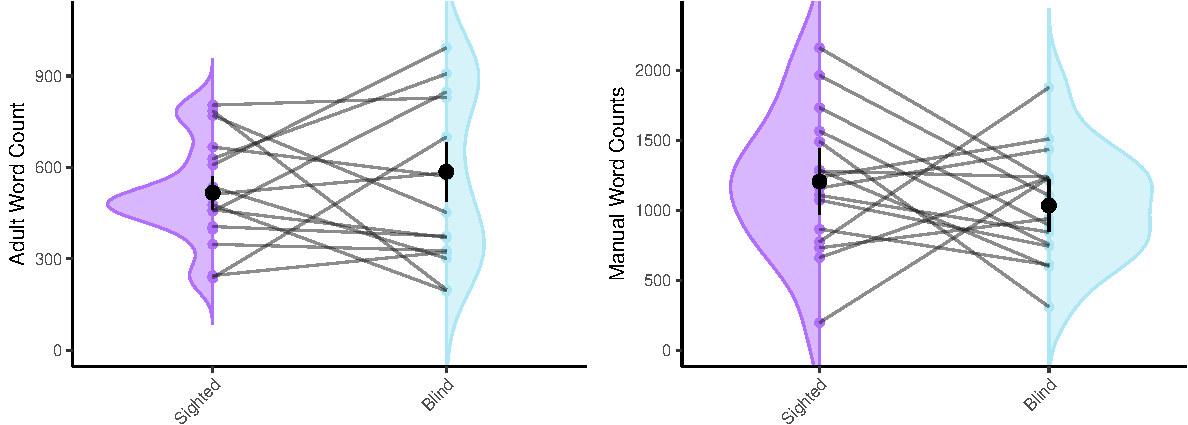
\includegraphics{input_quality_manuscript_files/figure-latex/quantity-plots-1.pdf}
\caption{\label{fig:quantity-plots}Comparing LENA-generated adult word counts (left) and transcription-based word counts in the input of blind and sighted children. Each dot represents the estimated number of words in one child's recording.}
\end{figure}

\hypertarget{interactivity-1}{%
\subsubsection{Interactivity}\label{interactivity-1}}

Next, we ask whether the language environments of blind vs.~sighted participants differ in the amount of interaction with the child, by comparing the proportion of child-directed speech and the number of conversational turns. Both measures were normally distributed (Prop. CDS: W = 0.97, \emph{p} = .969; CTC: W = 0.88, \emph{p} = .878). This set of analyses involves two tests, so our Bonferroni-corrected threshold for significance is \emph{p} \textless{} 0.03. Paired t-test revealed no significant difference in the proportion of child-directed speech (\emph{t} = 0.06, \emph{p} = .952) or in conversational turn counts to blind children versus to sighted children .

\begin{figure}
\centering
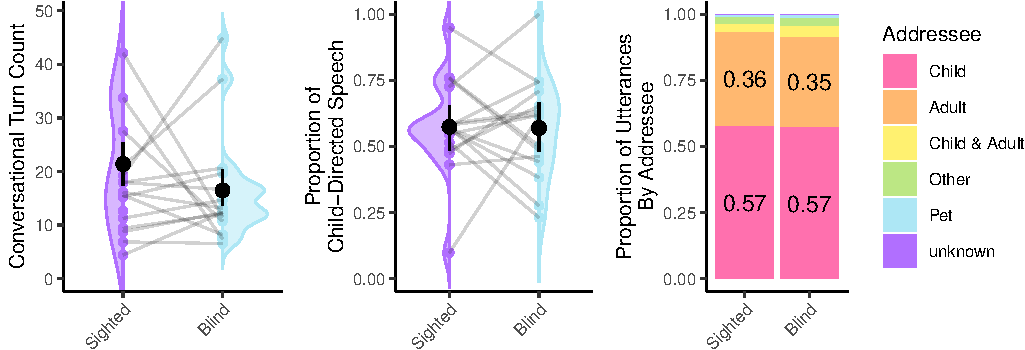
\includegraphics{input_quality_manuscript_files/figure-latex/interactivity-plots-1.pdf}
\caption{\label{fig:interactivity-plots}Comparing LENA-generated conversational turn counts (left) and proportion of utterances in child-directed speech (center). Each dot represents one child's recording. The full breakdown by addressee is shown in the rightmost panel.}
\end{figure}

\hypertarget{linguistic-features-1}{%
\subsubsection{Linguistic Features}\label{linguistic-features-1}}

\begin{figure}
\centering
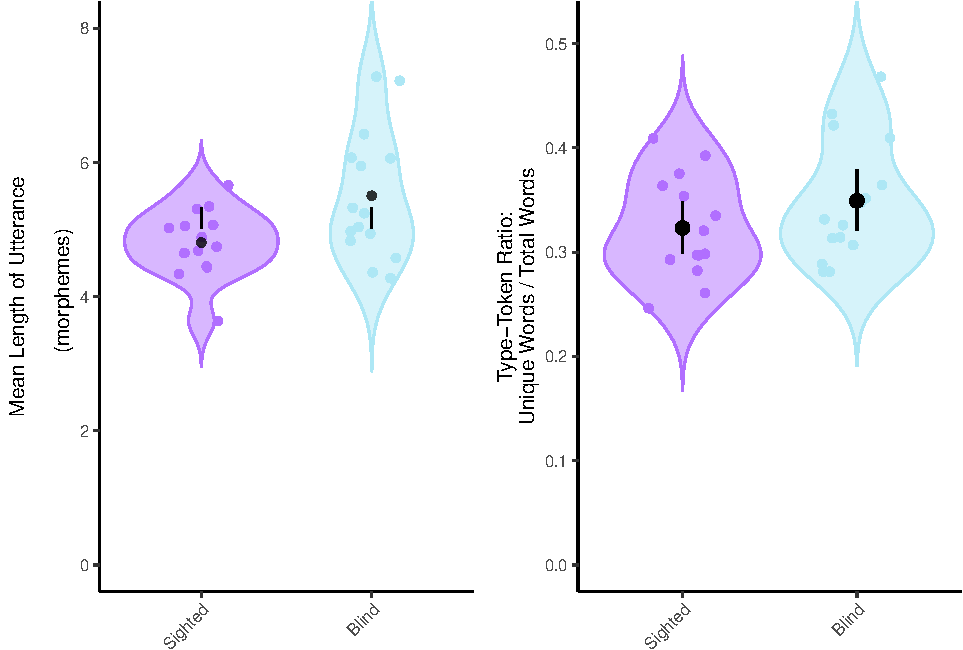
\includegraphics{input_quality_manuscript_files/figure-latex/linguistic-plots-1.pdf}
\caption{\label{fig:linguistic-plots}Comparing linguistic features: Mean length of utterance (left); each dot represents one speaker. Type-token ratio (right). Each dot represents one child's recording.}
\end{figure}

For linguistic features, we measure type-token ratio and mean length of utterance, two variables derived from the manual annotations. Because these variables met the normality assumption (TTR: W = 0.97, \emph{p} = .965; MLU: (W = 0.94, \emph{p} = .937)), we performed paired t-tests. Again, Bonferroni-corrected significance was set to \emph{p} \textless{} 0.03. Results indicated that there was no significant difference in type-token ratio between the two groups (\emph{t}(15) = -2.25, \emph{p} = .040), but that for MLU, utterances were slightly longer to blind children than to their sighted peers (\emph{t}(15) = -2.51, \emph{p} = .024); see Figure \ref{fig:linguistic-plots}).

\hypertarget{conceptual-features-1}{%
\subsubsection{Conceptual Features}\label{conceptual-features-1}}

Lastly, we compared three measures of the conceptual features of language input: the proportion of temporally displaced verbs, the distribution of Child-Body-Object Interaction ratings across words in the input, and the proportion of highly visual words. This set of analyses involves three tests, so our Bonferroni-corrected threshold for significance is \emph{p} \textless{} 0.02. Because the proportion of displaced verbs does not follow a normal distribution (W = 0.96, \emph{p} = .960), we tested this measure with a paired Wilcoxon test: we find that blind children hear proportionally more displaced verbs than sighted children (\emph{W} = 24, \emph{p} = .021). Next, we compared the distribution of CBOI ratings in word tokens in blind children's input to that in sighted children's input using a two-sample Kilgomorov-Smirnov test. These distributions significantly differ (D = 0.98, \emph{p} \textless{} .001). Descriptively, low CBOI words were more common in language input to blind children, and high CBOI words were more common in language input to sighted children; see Figure \ref{fig:conceptual-plots}. For the proportion of highly visual words, a Shapiro-Wilks test showed that this variable was normally distributed (W = 0.88, \emph{p} = .880). A paired t-test found no significant difference across groups in the proportion of highly visual words (\emph{t}(15) = 0.80, \emph{p} = .439).

\begin{table}

\caption{\label{tab:ps}Summary of analyses over language input variables.}
\centering
\fontsize{9}{11}\selectfont
\begin{tabular}[t]{>{\raggedright\arraybackslash}p{1.1in}|>{\raggedright\arraybackslash}p{1.2in}|>{\raggedright\arraybackslash}p{.45in}|>{\centering\arraybackslash}p{.7in}}
\hline
Variable & Direction & p value & Survives Bonferroni Correction?\\
\hline
Adult Word Count & Blind \textasciitilde{} Sighted & .245 & \\
\hline
Manual Word Count & Blind \textasciitilde{} Sighted & .294 & \\
\hline
Prop. Child-Directed Speech & Blind \textasciitilde{} Sighted & .952 & \\
\hline
Conversational Turn Count & Blind \textasciitilde{} Sighted & .096 & \\
\hline
Type-Token Ratio & Blind > Sighted & .040* & \\
\hline
Mean Length of Utterance & Blind > Sighted & .024* & *\\
\hline
Prop. Displaced & Blind > Sighted & .021* & \\
\hline
Child-Body-Object Interaction & Blind < Sighted & < .001* & *\\
\hline
Prop. Visual & Blind \textasciitilde{} Sighted & .439 & \\
\hline
\end{tabular}
\end{table}

\hypertarget{discussion}{%
\section{Discussion}\label{discussion}}

This study, which contains more blind participants than prior research alongside a carefully peer-matched sighted sample, measured language input to young blind children and their sighted peers, using the LENA audio recorder to capture naturalistic speech in the home. We found that across many dimensions of language input, parents largely talk similarly to blind and sighted children, with a few nuanced differences, that we discuss further below.

\hypertarget{quantity-1}{%
\subsection{Quantity}\label{quantity-1}}

Across two measures of language input quantity, one estimated from the full sixteen hour recording (Adult Word Count) and one precisely measured from a 30-minute window of that day (Manual Word Count), blind and sighted children were exposed to similar amounts of speech in the home. Quantity was highly variable \emph{within} groups, but we found no evidence for \emph{between} group differences in input quantity. This runs counter to two folk accounts of language input to blind children: 1) that sighted parents of blind children might talk \emph{less} because they don't share visual common ground with their children; 2) that parents of blind children might talk \emph{more} to compensate for their children's lack of visual input. Instead, we find a similar quantity of speech across groups.

\hypertarget{interactivity-2}{%
\subsection{Interactivity}\label{interactivity-2}}

We quantified interactivity in two ways: through the LENA-estimated conversational turn count and through the proportion of child-directed speech in our manual annotations. Again, we found no differences across groups in the amount of parent-child interaction. This finding contrasts with previous research; other studies report \emph{less} interaction in dyads where the child is blind (Pérez-Pereira \& Conti-Ramsden, 2001; Rowland, 1984; Andersen et al., 1993; Grumi et al., 2021; Kekelis \& Andersen, 1984;, Moore \& McConachie, 1994; Preisler, 1991). Using a non-visual sampling method (i.e., our audio recordings) might provide a different, more naturalistic perspective on parent-child interactions, particularly in this population. For one thing, many prior studies (e.g., Kekelis \& Andersen, 1984; Moore \& McConachie, 1994; Pérez-Pereira \& Conti-Ramsden, 2001; Preisler, 1991) involve video recordings in the child's home, with the researcher present. Like other young children, blind children distinguish between familiar individuals and strangers, and react with trepidation to the presence of a stranger (Fraiberg, 1975; McRae, 2002); for blind children, this reaction may involve ``quieting'', wherein children cease speaking or vocalizing when they hear a new voice in the home (Fraiberg, 1975; McRae, 2002). By having a researcher present during the recordings\footnote{Fraiberg (1975) writes ``these fear and avoidance behaviors appear even though the observer, a twice-monthly visitor, is not, strictly speaking, a stranger.'' (pg. 323).} , prior research may have artificially suppressed blind children's initiation of interactions. Even naturalistic observer-free video-recordings appear to inflate aspects of parental input, relative to daylong recordings (Bergelson et al., 2019). In these cases, the video camera acts as an observer itself, making participants aware of its presence, limiting participants' mobility, and therefore shrinking the pragmatic scope of possible interactions. Together, these factors could explain why past parent-child interaction research finds that blind children initiate fewer interactions (Andersen et al., 1993; Dote-Kwan, 1995; Kekelis \& Andersen, 1984; Moore \& McConachie, 1994; Tröster \& Brambring, 1992), that parents do most of the talking (Andersen et al., 1993; Kekelis \& Andersen, 1984), and that there is overall less interaction (Nagayoshi et al., 2017; Sally J. Rogers \& Puchalski, 1984; Rowland, 1984; Tröster \& Brambring, 1992).

Additionally, a common focus in earlier interaction literature is to measure visual cues of interaction, such as shared gaze or attentiveness to facial expressions (Baird, Mayfield, \& Baker, 1997; Preisler, 1991; Sally J. Rogers \& Puchalski, 1984). We can't help but wonder: are visual markers of social interaction the right yardstick to measure blind children against? In line with MacLeod and Demers (2023), perhaps the field should move away from sighted indicators of interaction ``quality'', and instead situate blind children's interactions within their own developmental niche, one that may be better captured with auditory- or tactile-focused coding schemes.

\hypertarget{linguistic-features-2}{%
\subsection{Linguistic Features}\label{linguistic-features-2}}

Along the linguistic dimension, we measured type-token ratio and mean length of utterance. Type-token ratio was similar across groups and similar to type-token ratios reported in other child-centered corpora (e.g., Newman, Rowe, \& Bernstein Ratner, 2016), suggesting that blind and sighted children are exposed to similar amounts of lexical diversity.

For MLU, we expected to find lower MLU in language input to blind children relative to sighted children. Parents of children with disabilities (Chernyak, n.d.; including parents of blind children! e.g., FamilyConnect, n.d.) are often advised to use shorter, simpler sentences with their children, and correspondingly, previous work finds that parents of children with disabilities tend to find that parents use shorter, simpler utterances (e.g., Down syndrome, Lorang, Venker, \& Sterling, 2020; hearing loss, Dirks et al., 2020). In many cases, however, this advice is not supported by the literature; evidence suggests that longer, more complex utterances are associated with better child language outcomes in both typically-developing children (Hoff \& Naigles, 2002) and children with cognitive differences (Sandbank \& Yoder, 2016). In our sample, we found similar (and perhaps even \emph{higher}) MLUs in blind children's language environment, relative to sighted children. If anything, the language environments of blind children trend towards \emph{longer}, more complex utterances.

\hypertarget{conceptual-features-2}{%
\subsection{Conceptual Features}\label{conceptual-features-2}}

Relative to other aspects of language input, the conceptual dimension varied most across groups. Although there are many potential ways to measure the conceptual features of language, we chose to capture \emph{here-and-now}-ness by measuring the proportion of temporally displaced verbs, the distribution of high vs.~low child-body-object interaction ratings for content words, and the proportion of highly visual words. Though blind and sighted participants were exposed to a similar proportion of highly visual words, blind children heard more temporally displaced verbs and their content words were distributed slightly more to the ``not-interactable'' end of the child-body-object interaction scale.

The extent to which blind children's language input is centered on the \emph{here-and-now} has been contested in the literature (Andersen et al., 1993; J. Campbell, 2003; Kekelis \& Andersen, 1984; Moore \& McConachie, 1994; Urwin, 1984). This aspect of language input is of particular interest because, for sighted children, decontextualized language in the input is associated with children's own use of decontextualized language, and early reports suggest that blind children's own use of decontextualized language develops later than sighted children's\footnote{Perhaps relatedly, object permanence and related skills may be delayed in blind children, S. J. Rogers and Puchalski (1988).} (A. Bigelow, 1990; Urwin, 1984). Could this be related to an absence of decontextualized language in the input? Our sample says no: we find that blind children's input contains \emph{more} decontextualized language. One possible explanation is that because children have less access to immediate visual cues, caregivers might instead refer to past or future events to engage with their child. To illustrate, while riding on a train, instead of describing the scenery passing outside the window, parents may choose to talk about what happened earlier in the day or their plans upon home. Without further information about the social and perceptual context, it is difficult to determine the communicative function of the differences we find in conceptual features we find or how they might explain differences in children's decontextualized language use. As more dense annotation becomes available, we can explore the social and environmental contexts of conceptual information as it unfolds across discourse.

\hypertarget{patterns-in-language-input}{%
\subsection{Patterns in Language Input}\label{patterns-in-language-input}}

Before synthesizing an account of these differences, we wish to highlight again how much variability there is \emph{within} groups and how much consistency there is \emph{between} groups. One could imagine a world in which the language environments of blind and sighted children are radically different from each other. Our data do not support that hypothesis. Rather, we find far more similarity across groups than differences, and all differences were small in magnitude. This is worth emphasizing and re-emphasizing: across developmental contexts, including, as we show here, visual experience, children's language input is resoundingly similar (Bergelson et al., 2022).

When we zoom into more fine-grained aspects of the input, we find that blind children's language environments contain longer utterances, more temporal displacement, and content words that are harder for children to interact with. Together, these features suggest that blind toddlers' input is more similar to speech directed towards older children or adults (Rowe, 2012; Snow, 1972) than sighted toddlers'. We cannot singularly attribute this to differences in addressee: our manual annotations indicate a similar proportion of child-.vs.adult-directed speech across the two groups.

One explanation for the (minimal) differences between blind and sighted children's language environments is parents' ability to assess their children's engagement and cognitive level, and thereby tailor their speech accordingly. Sighted parents may be less readily able to recognize blind children's signals of interest (Perez-Pereira \& Conti-Ramsden, 1999), and as a result, may respond less often to infants' vocalizations and bids for communication (Rowland, 1984), instead defaulting to more adultlike language.

\hypertarget{connecting-to-language-outcomes}{%
\subsection{Connecting to Language Outcomes}\label{connecting-to-language-outcomes}}

Returning to the larger equation of language development, blind and sighted infants differ in their access to perceptual input, and we have shown that language input is different along only a few axes: conceptual features, where language and the perceptual world interact, and complexity, with blind children hearing slightly longer and more adult-like utterances, on average. Initial vocabulary delays in blind children may then primarily be a result of the conflict between their lack of visual access and the majority-visual cues to early ``brute-force'' word learning (e.g., shared gaze, pointing, visual perception of referents). It could be precisely this linguistic input complexity which aids blind children in acquiring semantic knowledge later in development, once the first words are acquired. Under this theory, language input interventions or specific compensatory strategies for input to blind children become unnecessary for cognitively-typical blind children: the rich information in the language input and the infants' own learning capacity are plenty sufficient for acquiring language. Testing this prediction awaits further research.

\hypertarget{conclusion}{%
\section{Conclusion}\label{conclusion}}

In summary, our study compared language input in homes of 15 blind and 15 sighted infants/toddlers. We found that both groups received similar quantities of adult speech and had similar levels of interaction. However, blind children were exposed to longer utterances and more decontextualized language, suggesting that they are being exposed to a rich and complex linguistic environment that differs from the language input of sighted children. Our study does not imply that parents should change their communication styles, but rather highlights the importance of recognizing and appreciating the unique language experiences of blind children. Future research could investigate how these input differences impact the language development and cognitive abilities of blind and sighted children alike.

\hypertarget{references}{%
\section*{References}\label{references}}
\addcontentsline{toc}{section}{References}

\hypertarget{refs}{}
\begin{CSLReferences}{1}{0}
\leavevmode\vadjust pre{\hypertarget{ref-andersen1993}{}}%
Andersen, E. S., Dunlea, A., \& Kekelis, L. (1993). The impact of input: Language acquisition in the visually impaired. \emph{First Language}, \emph{13}(37), 23--49. \url{https://doi.org/10.1177/014272379301303703}

\leavevmode\vadjust pre{\hypertarget{ref-anderson2021}{}}%
Anderson, N. J., Graham, S. A., Prime, H., Jenkins, J. M., \& Madigan, S. (2021). Linking {Quality} and {Quantity} of {Parental Linguistic Input} to {Child Language Skills}: {A Meta-Analysis}. \emph{Child Development}, \emph{92}(2), 484--501. \url{https://doi.org/10.1111/cdev.13508}

\leavevmode\vadjust pre{\hypertarget{ref-babineau2021}{}}%
Babineau, M., de Carvalho, A., Trueswell, J., \& Christophe, A. (2021). Familiar words can serve as a semantic seed for syntactic bootstrapping. \emph{Developmental Science}, \emph{24}(1), e13010. \url{https://doi.org/10.1111/desc.13010}

\leavevmode\vadjust pre{\hypertarget{ref-babineau2022}{}}%
Babineau, M., Havron, N., Dautriche, I., de Carvalho, A., \& Christophe, A. (2022). Learning to predict and predicting to learn: {Before} and beyond the syntactic bootstrapper. \emph{Language Acquisition}, \emph{0}(0), 1--24. \url{https://doi.org/10.1080/10489223.2022.2078211}

\leavevmode\vadjust pre{\hypertarget{ref-baird1997}{}}%
Baird, S. M., Mayfield, P., \& Baker, P. (1997). Mothers' {Interpretations} of the {Behavior} of {Their Infants} with {Visual} and {Other Impairments} during {Interactions}. \emph{Journal of Visual Impairment \& Blindness}, \emph{91}(5), 467--483. \url{https://doi.org/10.1177/0145482X9709100507}

\leavevmode\vadjust pre{\hypertarget{ref-bergelson2019}{}}%
Bergelson, E., Amatuni, A., Dailey, S., Koorathota, S., \& Tor, S. (2019). Day by day, hour by hour: {Naturalistic} language input to infants. \emph{Developmental Science}, \emph{22}(1), e12715. \url{https://doi.org/10.1111/desc.12715}

\leavevmode\vadjust pre{\hypertarget{ref-bergelson2022a}{}}%
Bergelson, E., Soderstrom, M., Schwarz, I.-C., Rowland, C., Ramirez-Esparza, N., Hamrick, L., \ldots{} Casillas, M. (2022). Everyday language input and production in 1001 children from 6 continents.

\leavevmode\vadjust pre{\hypertarget{ref-bergelson2013}{}}%
Bergelson, E., \& Swingley, D. (2013). The acquisition of abstract words by young infants. \emph{Cognition}, \emph{127}(3), 391--397. \url{https://doi.org/10.1016/j.cognition.2013.02.011}

\leavevmode\vadjust pre{\hypertarget{ref-bernsteinratner1984}{}}%
Bernstein Ratner, N. (1984). Patterns of vowel modification in mother\textendash child speech. \emph{Journal of Child Language}, \emph{11}, 557--578.

\leavevmode\vadjust pre{\hypertarget{ref-bigelow1987}{}}%
Bigelow, Ann. (1987). Early words of blind children. \emph{Journal of Child Language}, \emph{14}(1), 47--56. \url{https://doi.org/10.1017/S0305000900012721}

\leavevmode\vadjust pre{\hypertarget{ref-bigelow1990}{}}%
Bigelow, A. (1990). Relationship between the {Development} of {Language} and {Thought} in {Young Blind Children}. \emph{Journal of Visual Impairment \& Blindness}, \emph{84}(8), 414--419. \url{https://doi.org/10.1177/0145482X9008400805}

\leavevmode\vadjust pre{\hypertarget{ref-bratt2022}{}}%
Bratt, J., Harmon, J., \& Learning, B. F. \&. W. P. G. L. D. M. (2022). Morphemepiece: {Morpheme Tokenization}.

\leavevmode\vadjust pre{\hypertarget{ref-brugman2009}{}}%
Brugman, H., \& Russel, A. (2009). Annotating {Multimedia} / {Multi-modal} resources with {ELAN}. \emph{Proceedings of the Fourth International Conference on Language Resources and Evaluation}.

\leavevmode\vadjust pre{\hypertarget{ref-busch2018}{}}%
Busch, T., Sangen, A., Vanpoucke, F., \& van Wieringen, A. (2018). Correlation and agreement between {Language ENvironment Analysis} ({LENA}\texttrademark ) and manual transcription for {Dutch} natural language recordings. \emph{Behavior Research Methods}, \emph{50}(5), 1921--1932. \url{https://doi.org/10.3758/s13428-017-0960-0}

\leavevmode\vadjust pre{\hypertarget{ref-campbell2022}{}}%
Campbell, E. E., \& Bergelson, E. (2022). Making sense of sensory language: {Acquisition} of sensory knowledge by individuals with congenital sensory impairments. \emph{Neuropsychologia}, \emph{174}, 108320. \url{https://doi.org/10.1016/j.neuropsychologia.2022.108320}

\leavevmode\vadjust pre{\hypertarget{ref-campbellsubmitted}{}}%
Campbell, E. E., Casillas, R., \& Bergelson, E. (submitted). The {Role} of {Vision} in the {Acquisition} of {Words}: {Vocabulary Development} in {Blind Toddlers}. \url{https://doi.org/10.17605/OSF.IO/UW6ZM}

\leavevmode\vadjust pre{\hypertarget{ref-campbell2003}{}}%
Campbell, J. (2003). Maternal {Directives} to {Young Children} who are {Blind}. \emph{Journal of Visual Impairment \& Blindness}, \emph{97}(6), 355--365. \url{https://doi.org/10.1177/0145482X0309700604}

\leavevmode\vadjust pre{\hypertarget{ref-casillas2020}{}}%
Casillas, M., Brown, P., \& Levinson, S. C. (2020). Early {Language Experience} in a {Tseltal Mayan Village}. \emph{Child Development}, \emph{91}(5), 1819--1835. \url{https://doi.org/10.1111/cdev.13349}

\leavevmode\vadjust pre{\hypertarget{ref-chernyak}{}}%
Chernyak, P. (n.d.). 3 {Ways} to {Teach Your Blind} or {Visually Impaired Child} to {Talk}. \emph{WikiHow}. https://www.wikihow.life/Teach-Your-Blind-or-Visually-Impaired-Child-to-Talk.

\leavevmode\vadjust pre{\hypertarget{ref-chiesa2015}{}}%
Chiesa, S., Galati, D., \& Schmidt, S. (2015). Communicative interactions between visually impaired mothers and their sighted children: Analysis of gaze, facial expressions, voice and physical contacts. \emph{Child: Care, Health and Development}, \emph{41}(6), 1040--1046. \url{https://doi.org/10.1111/cch.12274}

\leavevmode\vadjust pre{\hypertarget{ref-cychosz2021a}{}}%
Cychosz, M., Villanueva, A., \& Weisleder, A. (2021). Efficient {Estimation} of {Children}'s {Language Exposure} in {Two Bilingual Communities}. \emph{Journal of Speech, Language, and Hearing Research}, \emph{64}(10), 3843--3866. \url{https://doi.org/10.1044/2021_JSLHR-20-00755}

\leavevmode\vadjust pre{\hypertarget{ref-devilliers1985}{}}%
De Villiers, J. (1985). Learning how to use verbs: Lexical coding and the influence of the input*. \emph{Journal of Child Language}, \emph{12}(3), 587--595. \url{https://doi.org/10.1017/S0305000900006668}

\leavevmode\vadjust pre{\hypertarget{ref-demir2015}{}}%
Demir, Ö. E., Rowe, M. L., Heller, G., Goldin-Meadow, S., \& Levine, S. C. (2015). Vocabulary, syntax, and narrative development in typically developing children and children with early unilateral brain injury: Early parental talk about the "there-and-then" matters. \emph{Developmental Psychology}, \emph{51}(2), 161--175. \url{https://doi.org/10.1037/a0038476}

\leavevmode\vadjust pre{\hypertarget{ref-dirks2020}{}}%
Dirks, E., Stevens, A., Kok, S., Frijns, J., \& Rieffe, C. (2020). Talk with me! {Parental} linguistic input to toddlers with moderate hearing loss. \emph{Journal of Child Language}, \emph{47}(1), 186--204. \url{https://doi.org/10.1017/S0305000919000667}

\leavevmode\vadjust pre{\hypertarget{ref-donnellan2020}{}}%
Donnellan, E., Bannard, C., McGillion, M. L., Slocombe, K. E., \& Matthews, D. (2020). Infants' intentionally communicative vocalizations elicit responses from caregivers and are the best predictors of the transition to language: {A} longitudinal investigation of infants' vocalizations, gestures and word production. \emph{Developmental Science}, \emph{23}(1), e12843. \url{https://doi.org/10.1111/desc.12843}

\leavevmode\vadjust pre{\hypertarget{ref-dote-kwan1995}{}}%
Dote-Kwan, J. (1995). Impact of {Mothers}' {Interactions} on the {Development} of {Their Young Visually Impaired Children}. \emph{Journal of Visual Impairment \& Blindness}, \emph{89}(1), 46--58. \url{https://doi.org/10.1177/0145482X9508900109}

\leavevmode\vadjust pre{\hypertarget{ref-familyconnect}{}}%
FamilyConnect. (n.d.). Understanding the {Stages} of {Language Development} for {Babies Who Are Blind}. \emph{FamilyConnect}.

\leavevmode\vadjust pre{\hypertarget{ref-fenson1994}{}}%
Fenson, L., Dale, P. S., Reznick, J. S., Bates, E., Thal, D. J., Pethick, S. J., \ldots{} Stiles, J. (1994). Variability in {Early Communicative Development}. \emph{Monographs of the Society for Research in Child Development}, \emph{59}(5), i. \url{https://doi.org/10.2307/1166093}

\leavevmode\vadjust pre{\hypertarget{ref-ferjanramirez2021}{}}%
Ferjan Ramírez, N., Hippe, D. S., \& Kuhl, P. K. (2021). Comparing {Automatic} and {Manual Measures} of {Parent}\textendash{{Infant Conversational Turns}}: {A Word} of {Caution}. \emph{Child Development}, \emph{92}(2), 672--681. \url{https://doi.org/10.1111/cdev.13495}

\leavevmode\vadjust pre{\hypertarget{ref-fernald1989}{}}%
Fernald, A. (1989). \href{https://www.ncbi.nlm.nih.gov/pubmed/2612255}{Intonation and communicative intent in mothers' speech to infants: Is the melody the message?} \emph{Child Development}, \emph{60}(6), 1497--1510.

\leavevmode\vadjust pre{\hypertarget{ref-fraiberg1975}{}}%
Fraiberg, S. (1975). The development of human attachments in infants blind from birth. \emph{Merrill-Palmer Quarterly}, \emph{21}, 315--334.

\leavevmode\vadjust pre{\hypertarget{ref-ganea2018}{}}%
Ganea, N., Hudry, K., Vernetti, A., Tucker, L., Charman, T., Johnson, M. H., \& Senju, A. (2018). Development of adaptive communication skills in infants of blind parents. \emph{Developmental Psychology}, \emph{54}(12), 2265--2273. \url{https://doi.org/10.1037/dev0000564}

\leavevmode\vadjust pre{\hypertarget{ref-ganea2013}{}}%
Ganea, P. A., \& Saylor, M. M. (2013). Talking about the near and dear: {Infants}' comprehension of displaced speech. \emph{Developmental Psychology}, \emph{49}(7), 1299--1307. \url{https://doi.org/10.1037/a0030086}

\leavevmode\vadjust pre{\hypertarget{ref-ganek2016}{}}%
Ganek, H., \& Eriks-Brophy, A. (2016). The {Language ENvironment Analysis} ({LENA}) system: {A} literature review. In \emph{Proceedings of the joint workshop on {NLP} for {Computer Assisted Language Learning} and {NLP} for {Language Acquisition}} (pp. 24--32). {Umeå, Sweden}: {LiU Electronic Press}.

\leavevmode\vadjust pre{\hypertarget{ref-ganek2018}{}}%
Ganek, H., \& Eriks-Brophy, A. (2018). Language {ENvironment} analysis ({LENA}) system investigation of day long recordings in children: {A} literature review. \emph{Journal of Communication Disorders}, \emph{72}, 77--85. \url{https://doi.org/10.1016/j.jcomdis.2017.12.005}

\leavevmode\vadjust pre{\hypertarget{ref-gergle2004}{}}%
Gergle, D., Kraut, R. E., \& Fussell, S. R. (2004). Language {Efficiency} and {Visual Technology}: {Minimizing Collaborative Effort} with {Visual Information}. \emph{Journal of Language and Social Psychology}, \emph{23}(4), 491--517. \url{https://doi.org/10.1177/0261927X04269589}

\leavevmode\vadjust pre{\hypertarget{ref-gilkerson2008}{}}%
Gilkerson, J., \& Richards, J. A. (2008). \emph{The {LENA Natural Language Study}}. {Boulder, CO}: {LENA Foundation}.

\leavevmode\vadjust pre{\hypertarget{ref-gilkerson2018}{}}%
Gilkerson, J., Richards, J. A., Warren, S. F., Oller, D. K., Russo, R., \& Vohr, B. (2018). Language {Experience} in the {Second Year} of {Life} and {Language Outcomes} in {Late Childhood}. \emph{Pediatrics}, \emph{142}(4), e20174276. \url{https://doi.org/10.1542/peds.2017-4276}

\leavevmode\vadjust pre{\hypertarget{ref-gleitman1990}{}}%
Gleitman, L. (1990). The {Structural Sources} of {Verb Meanings}. \emph{Language Acquisition}, \emph{1}(1), 3--55. Retrieved from \url{https://www.jstor.org/stable/20011341}

\leavevmode\vadjust pre{\hypertarget{ref-goldstein2008}{}}%
Goldstein, M. H., \& Schwade, J. A. (2008). Social feedback to infants' babbling facilitates rapid phonological learning. \emph{Psychological Science}, \emph{19}(5), 515--523. \url{https://doi.org/10.1111/j.1467-9280.2008.02117.x}

\leavevmode\vadjust pre{\hypertarget{ref-grice1975}{}}%
Grice, H. P. (1975). {Logic and Conversation}. In \emph{{Syntax and semantics}}. {New York San Francisco London}: {Academic press, Harcourt Brace Jovanovich}.

\leavevmode\vadjust pre{\hypertarget{ref-grigoroglou2016}{}}%
Grigoroglou, M., Edu, U., \& Papafragou, A. (2016). Are children flexible speakers? {Effects} of typicality and listener needs in children's event descriptions. \emph{Cognitive Science}, 6.

\leavevmode\vadjust pre{\hypertarget{ref-grimminger2020}{}}%
Grimminger, A., Rohlfing, K. J., Lüke, C., Liszkowski, U., \& Ritterfeld, U. (2020). Decontextualized talk in caregivers' input to 12-month-old children during structured interaction. \emph{Journal of Child Language}, \emph{47}(2), 418--434. \url{https://doi.org/10.1017/S0305000919000710}

\leavevmode\vadjust pre{\hypertarget{ref-grumi2021}{}}%
Grumi, S., Cappagli, G., Aprile, G., Mascherpa, E., Gori, M., Provenzi, L., \& Signorini, S. (2021). Togetherness, beyond the eyes: {A} systematic review on the interaction between visually impaired children and their parents. \emph{Infant Behavior and Development}, \emph{64}, 101590. \url{https://doi.org/10.1016/j.infbeh.2021.101590}

\leavevmode\vadjust pre{\hypertarget{ref-hadley2017}{}}%
Hadley, P. A., Rispoli, M., Holt, J. K., Papastratakos, T., Hsu, N., Kubalanza, M., \& McKenna, M. M. (2017). Input {Subject Diversity Enhances Early Grammatical Growth}: {Evidence} from a {Parent-Implemented Intervention}. \emph{Language Learning and Development: The Official Journal of the Society for Language Development}, \emph{13}(1), 54--79. \url{https://doi.org/10.1080/15475441.2016.1193020}

\leavevmode\vadjust pre{\hypertarget{ref-harris1986}{}}%
Harris, M., Jones, D., Brookes, S., \& Grant, J. (1986). Relations between the non-verbal context of maternal speech and rate of language development. \emph{British Journal of Developmental Psychology}, \emph{4}(3), 261--268. \url{https://doi.org/10.1111/j.2044-835X.1986.tb01017.x}

\leavevmode\vadjust pre{\hypertarget{ref-hawkins2021}{}}%
Hawkins, R. D., Gweon, H., \& Goodman, N. D. (2021). The {Division} of {Labor} in {Communication}: {Speakers Help Listeners Account} for {Asymmetries} in {Visual Perspective}. \emph{Cognitive Science}, \emph{45}(3), e12926. \url{https://doi.org/10.1111/cogs.12926}

\leavevmode\vadjust pre{\hypertarget{ref-hazan2011}{}}%
Hazan, V., \& Baker, R. (2011). Acoustic-phonetic characteristics of speech produced with communicative intent to counter adverse listening conditions. \emph{The Journal of the Acoustical Society of America}, \emph{130}(4), 2139--2152. \url{https://doi.org/10.1121/1.3623753}

\leavevmode\vadjust pre{\hypertarget{ref-hirsh-pasek2015}{}}%
Hirsh-Pasek, K., Adamson, L. B., Bakeman, R., Owen, M. T., Golinkoff, R. M., Pace, A., \ldots{} Suma, K. (2015). The {Contribution} of {Early Communication Quality} to {Low-Income Children}'s {Language Success}. \emph{Psychological Science}, \emph{26}(7), 1071--1083. \url{https://doi.org/10.1177/0956797615581493}

\leavevmode\vadjust pre{\hypertarget{ref-hoff2003}{}}%
Hoff, E. (2003 Sep-Oct). The specificity of environmental influence: Socioeconomic status affects early vocabulary development via maternal speech. \emph{Child Development}, \emph{74}(5), 1368--1378. \url{https://doi.org/10.1111/1467-8624.00612}

\leavevmode\vadjust pre{\hypertarget{ref-hoff2002}{}}%
Hoff, E., \& Naigles, L. (2002). How children use input to acquire a lexicon. \emph{Child Development}, \emph{73}(2), 418--433. \url{https://doi.org/10.1111/1467-8624.00415}

\leavevmode\vadjust pre{\hypertarget{ref-hsu2017}{}}%
Hsu, N., Hadley, P. A., \& Rispoli, M. (2017). Diversity matters: Parent input predicts toddler verb production. \emph{Journal of Child Language}, \emph{44}(1), 63--86. \url{https://doi.org/10.1017/S0305000915000690}

\leavevmode\vadjust pre{\hypertarget{ref-hudson2002}{}}%
Hudson, J. A. (2002). "{Do You Know What We}'re {Going} to {Do This Summer}?": {Mothers}' {Talk} to {Preschool Children About Future Events}. \emph{Journal of Cognition and Development}, \emph{3}(1), 49--71. \url{https://doi.org/10.1207/S15327647JCD0301_4}

\leavevmode\vadjust pre{\hypertarget{ref-huttenlocher1991}{}}%
Huttenlocher, J., Haight, W., Bryk, A., Seltzer, M., \& Lyons, T. (1991). Early vocabulary growth: {Relation} to language input and gender. \emph{Developmental Psychology}, \emph{27}, 236--248. \url{https://doi.org/10.1037/0012-1649.27.2.236}

\leavevmode\vadjust pre{\hypertarget{ref-huttenlocher2002}{}}%
Huttenlocher, J., Vasilyeva, M., Cymerman, E., \& Levine, S. (2002). Language input and child syntax. \emph{Cognitive Psychology}, \emph{45}(3), 337--374. \url{https://doi.org/10.1016/s0010-0285(02)00500-5}

\leavevmode\vadjust pre{\hypertarget{ref-huttenlocher2010}{}}%
Huttenlocher, J., Waterfall, H., Vasilyeva, M., Vevea, J., \& Hedges, L. V. (2010). Sources of variability in children's language growth. \emph{Cognitive Psychology}, \emph{61}(4), 343--365. \url{https://doi.org/10.1016/j.cogpsych.2010.08.002}

\leavevmode\vadjust pre{\hypertarget{ref-jara-ettinger2021}{}}%
Jara-Ettinger, J., \& Rubio-Fernandez, P. (2021). The social basis of referential communication: {Speakers} construct physical reference based on listeners' expected visual search. \emph{Psychological Review}, No Pagination Specified--No Pagination Specified. \url{https://doi.org/10.1037/rev0000345}

\leavevmode\vadjust pre{\hypertarget{ref-kekelis1984}{}}%
Kekelis, L. S., \& Andersen, E. S. (1984). Family {Communication Styles} and {Language Development}. \emph{Journal of Visual Impairment \& Blindness}, \emph{78}(2), 54--65. \url{https://doi.org/10.1177/0145482X8407800202}

\leavevmode\vadjust pre{\hypertarget{ref-kramer1975}{}}%
Kramer, J. A., Hill, K. T., \& Cohen, L. B. (1975). Infants' {Development} of {Object Permanence}: {A Refined Methodology} and {New Evidence} for {Piaget}'s {Hypothesized Ordinality}. \emph{Child Development}, \emph{46}(1), 149--155. \url{https://doi.org/10.2307/1128843}

\leavevmode\vadjust pre{\hypertarget{ref-landau1985}{}}%
Landau, B., \& Gleitman, L. R. (1985). \emph{Language and experience: {Evidence} from the blind child} (pp. xi, 250). {Cambridge, MA, US}: {Harvard University Press}.

\leavevmode\vadjust pre{\hypertarget{ref-lavechin2021}{}}%
Lavechin, M., Bousbib, R., Bredin, H., Dupoux, E., \& Cristia, A. (2021). An open-source voice type classifier for child-centered daylong recordings. {arXiv}. \url{https://doi.org/10.48550/arXiv.2005.12656}

\leavevmode\vadjust pre{\hypertarget{ref-lehet2021}{}}%
Lehet, M., Arjmandi, M. K., Houston, D., \& Dilley, L. (2021). Circumspection in using automated measures: {Talker} gender and addressee affect error rates for adult speech detection in the {Language ENvironment Analysis} ({LENA}) system. \emph{Behavior Research Methods}, \emph{53}(1), 113--138. \url{https://doi.org/10.3758/s13428-020-01419-y}

\leavevmode\vadjust pre{\hypertarget{ref-lorang2020}{}}%
Lorang, E., Venker, C. E., \& Sterling, A. (2020). An investigation into maternal use of telegraphic input to children with {Down} syndrome. \emph{Journal of Child Language}, \emph{47}(1), 225--249. \url{https://doi.org/10.1017/S0305000919000503}

\leavevmode\vadjust pre{\hypertarget{ref-lucariello1987}{}}%
Lucariello, J., \& Nelson, K. (1987). Remembering and planning talk between mothers and children. \emph{Discourse Processes}, \emph{10}(3), 219--235. \url{https://doi.org/10.1080/01638538709544673}

\leavevmode\vadjust pre{\hypertarget{ref-lucca2018}{}}%
Lucca, K., \& Wilbourn, M. P. (2018). Communicating to {Learn}: {Infants}' {Pointing Gestures Result} in {Optimal Learning}. \emph{Child Development}, \emph{89}(3), 941--960. \url{https://doi.org/10.1111/cdev.12707}

\leavevmode\vadjust pre{\hypertarget{ref-luchkina2020}{}}%
Luchkina, E., Xu, F., Sobel, D., \& Morgan, J. (2020). \emph{Sixteen-month-olds comprehend unanchored absent reference} (Preprint). {Open Science Framework}. \url{https://doi.org/10.31219/osf.io/5tc6d}

\leavevmode\vadjust pre{\hypertarget{ref-lynott2020}{}}%
Lynott, D., Connell, L., Brysbaert, M., Brand, J., \& Carney, J. (2020). The {Lancaster Sensorimotor Norms}: Multidimensional measures of perceptual and action strength for 40,000 {English} words. \emph{Behavior Research Methods}, \emph{52}(3), 1271--1291. \url{https://doi.org/10.3758/s13428-019-01316-z}

\leavevmode\vadjust pre{\hypertarget{ref-macleod2023}{}}%
MacLeod, A. A. N., \& Demers, C. (2023). Transmitting white monolingual {Anglo-American} norms: {A} concept analysis of {``quality of language''} in parent-child interactions. \emph{Applied Psycholinguistics}, 1--29. \url{https://doi.org/10.1017/S014271642300005X}

\leavevmode\vadjust pre{\hypertarget{ref-macwhinney2019}{}}%
MacWhinney, B. (2019). {CHAT Manual}. \url{https://doi.org/10.21415/3MHN-0Z89}

\leavevmode\vadjust pre{\hypertarget{ref-magimairaj2022}{}}%
Magimairaj, B., Nagaraj, N., Caballero, A., Munoz, K., \& White, K. (2022). A {Systematic Review} of the {Effects} of {LENA-based Feedback} on {Parent-Child Language Interactions} in {Families} with {Young Children}. \emph{Journal of Early Hearing Detection and Intervention}, \emph{7}(3), 47--60. \url{https://doi.org/10.26077/6c72-973b}

\leavevmode\vadjust pre{\hypertarget{ref-mcrae2002}{}}%
McRae, K. A. (2002). \emph{Attachment in blind infants : A systematic investigation using {Ainsworth}'s {Strange Situation}.} (PhD thesis). University of Toronto, {Toronto, Canada}.

\leavevmode\vadjust pre{\hypertarget{ref-montag2018}{}}%
Montag, J. L., Jones, M. N., \& Smith, L. B. (2018). Quantity and {Diversity}: {Simulating Early Word Learning Environments}. \emph{Cognitive Science}, \emph{42 Suppl 2}(Suppl 2), 375--412. \url{https://doi.org/10.1111/cogs.12592}

\leavevmode\vadjust pre{\hypertarget{ref-moore1994}{}}%
Moore, V., \& McConachie, H. (1994). Communication between blind and severely visually impaired children and their parents. \emph{British Journal of Developmental Psychology}, \emph{12}(4), 491--502. \url{https://doi.org/10.1111/j.2044-835X.1994.tb00650.x}

\leavevmode\vadjust pre{\hypertarget{ref-muraki2022}{}}%
Muraki, E. J., Siddiqui, I. A., \& Pexman, P. M. (2022). Quantifying children's sensorimotor experience: {Child} body-object interaction ratings for 3359 {English} words. \emph{Behavior Research Methods}, \emph{54}(6), 2864--2877. \url{https://doi.org/10.3758/s13428-022-01798-4}

\leavevmode\vadjust pre{\hypertarget{ref-nagayoshi2017}{}}%
Nagayoshi, M., Hirose, T., Toju, K., Suzuki, S., Okamitsu, M., Teramoto, T., \ldots{} Takeo, N. (2017). Related visual impairment to mother-infant interaction and development in infants with bilateral retinoblastoma. \emph{European Journal of Oncology Nursing: The Official Journal of European Oncology Nursing Society}, \emph{28}, 28--34. \url{https://doi.org/10.1016/j.ejon.2017.02.002}

\leavevmode\vadjust pre{\hypertarget{ref-naigles1998}{}}%
Naigles, L. R., \& Hoff-Ginsberg, E. (1998). Why are some verbs learned before other verbs? {Effects} of input frequency and structure on children's early verb use. \emph{Journal of Child Language}, \emph{25}(1), 95--120. \url{https://doi.org/10.1017/S0305000997003358}

\leavevmode\vadjust pre{\hypertarget{ref-newman2016}{}}%
Newman, R. S., Rowe, M. L., \& Bernstein Ratner, N. (2016). Input and uptake at 7 months predicts toddler vocabulary: The role of child-directed speech and infant processing skills in language development. \emph{Journal of Child Language}, \emph{43}(5), 1158--1173. \url{https://doi.org/10.1017/S0305000915000446}

\leavevmode\vadjust pre{\hypertarget{ref-osina2013}{}}%
Osina, M. A., Saylor, M. M., \& Ganea, P. A. (2013). When familiar is not better: 12-month-old infants respond to talk about absent objects. \emph{Developmental Psychology}, \emph{49}, 138--145. \url{https://doi.org/10.1037/a0027903}

\leavevmode\vadjust pre{\hypertarget{ref-ostarek2019}{}}%
Ostarek, M., Paridon, J. van, \& Montero-Melis, G. (2019). Sighted people's language is not helpful for blind individuals' acquisition of typical animal colors. \emph{Proceedings of the National Academy of Sciences}, \emph{116}(44), 21972--21973. \url{https://doi.org/10.1073/pnas.1912302116}

\leavevmode\vadjust pre{\hypertarget{ref-pancsofar2006}{}}%
Pancsofar, N., \& Vernon-Feagans, L. (2006). Mother and father language input to young children: {Contributions} to later language development. \emph{Journal of Applied Developmental Psychology}, \emph{27}(6), 571--587. \url{https://doi.org/10.1016/j.appdev.2006.08.003}

\leavevmode\vadjust pre{\hypertarget{ref-perez-pereira1999}{}}%
Perez-Pereira, M., \& Conti-Ramsden, G. (1999). \emph{Language {Development} and {Social Interaction} in {Blind Children}}. {London}: {Psychology Press}. \url{https://doi.org/10.4324/9780203776087}

\leavevmode\vadjust pre{\hypertarget{ref-perez-pereira2001}{}}%
Pérez-Pereira, M., \& Conti-Ramsden, G. (2001). The use of {Directives} in {Verbal Interactions} between {Blind Children} and their {Mothers}. \emph{Journal of Visual Impairment \& Blindness}, \emph{95}(3), 133--149. \url{https://doi.org/10.1177/0145482x0109500302}

\leavevmode\vadjust pre{\hypertarget{ref-pisani2021}{}}%
Pisani, S., Gautheron, L., \& Cristia, A. (2021). \emph{Long-form recordings: {From A} to {Z}}.

\leavevmode\vadjust pre{\hypertarget{ref-preisler1991}{}}%
Preisler, G. M. (1991). Early patterns of interaction between blind infants and their sighted mothers. \emph{Child: Care, Health and Development}, \emph{17}(2), 65--90. \url{https://doi.org/10.1111/j.1365-2214.1991.tb00680.x}

\leavevmode\vadjust pre{\hypertarget{ref-richards1987}{}}%
Richards, B. (1987). Type/{Token Ratios}: What do they really tell us? \emph{Journal of Child Language}, \emph{14}(2), 201. \url{https://doi.org/doi:10.1017/s0305000900012885}

\leavevmode\vadjust pre{\hypertarget{ref-roder2003}{}}%
Röder, B., Demuth, L., Streb, J., \& Rösler, F. (2003). Semantic and morpho-syntactic priming in auditory word recognition in congenitally blind adults. \emph{Language and Cognitive Processes}, \emph{18}(1), 1--20. \url{https://doi.org/10.1080/01690960143000407}

\leavevmode\vadjust pre{\hypertarget{ref-roder2000}{}}%
Röder, B., Rösler, F., \& Neville, H. J. (2000). Event-related potentials during auditory language processing in congenitally blind and sighted people. \emph{Neuropsychologia}, \emph{38}(11), 1482--1502. \url{https://doi.org/10.1016/S0028-3932(00)00057-9}

\leavevmode\vadjust pre{\hypertarget{ref-rogers1984}{}}%
Rogers, Sally J., \& Puchalski, C. B. (1984). Social {Characteristics} of {Visually Impaired Infants}' {Play}. \emph{Topics in Early Childhood Special Education}, \emph{3}(4), 52--56. \url{https://doi.org/10.1177/027112148400300409}

\leavevmode\vadjust pre{\hypertarget{ref-rogers1988}{}}%
Rogers, S. J., \& Puchalski, C. B. (1988). Development of {Object Permanence} in {Visually Impaired Infants}. \emph{Journal of Visual Impairment \& Blindness}, \emph{82}(4), 137--142. \url{https://doi.org/10.1177/0145482X8808200407}

\leavevmode\vadjust pre{\hypertarget{ref-romeo2018}{}}%
Romeo, R. R., Leonard, J. A., Robinson, S. T., West, M. R., Mackey, A. P., Rowe, M. L., \& Gabrieli, J. D. E. (2018). Beyond the 30-{Million-Word Gap}: {Children}'s {Conversational Exposure Is Associated With Language-Related Brain Function}. \emph{Psychological Science}, \emph{29}(5), 700--710. \url{https://doi.org/10.1177/0956797617742725}

\leavevmode\vadjust pre{\hypertarget{ref-roseberry2014}{}}%
Roseberry, S., Hirsh-Pasek, K., \& Golinkoff, R. M. (2014 May-Jun). Skype me! {Socially} contingent interactions help toddlers learn language. \emph{Child Development}, \emph{85}(3), 956--970. \url{https://doi.org/10.1111/cdev.12166}

\leavevmode\vadjust pre{\hypertarget{ref-rowe2008}{}}%
Rowe, M. L. (2008). Child-directed speech: Relation to socioeconomic status, knowledge of child development and child vocabulary skill*. \emph{Journal of Child Language}, \emph{35}(1), 185--205. \url{https://doi.org/10.1017/S0305000907008343}

\leavevmode\vadjust pre{\hypertarget{ref-rowe2012}{}}%
Rowe, M. L. (2012). A {Longitudinal Investigation} of the {Role} of {Quantity} and {Quality} of {Child-Directed Speech} in {Vocabulary Development}. \emph{Child Development}, \emph{83}(5), 1762--1774. \url{https://doi.org/10.1111/j.1467-8624.2012.01805.x}

\leavevmode\vadjust pre{\hypertarget{ref-rowe2013}{}}%
Rowe, M. L. (2013). Decontextualized {Language Input} and {Preschoolers}' {Vocabulary Development}. \emph{Seminars in Speech and Language}, \emph{34}(4), 260--266. \url{https://doi.org/10.1055/s-0033-1353444}

\leavevmode\vadjust pre{\hypertarget{ref-rowe2020}{}}%
Rowe, M. L., \& Snow, C. E. (2020). Analyzing input quality along three dimensions: Interactive, linguistic, and conceptual. \emph{Journal of Child Language}, \emph{47}(1), 5--21. \url{https://doi.org/10.1017/S0305000919000655}

\leavevmode\vadjust pre{\hypertarget{ref-rowland1984}{}}%
Rowland, C. (1984). Preverbal {Communication} of {Blind Infants} and {Their Mothers}. \emph{Journal of Visual Impairment \& Blindness}, \emph{78}(7), 297--302. \url{https://doi.org/10.1177/0145482X8407800701}

\leavevmode\vadjust pre{\hypertarget{ref-rubio-fernandez2019}{}}%
Rubio-Fernandez, P. (2019). Overinformative {Speakers Are Cooperative}: {Revisiting} the {Gricean Maxim} of {Quantity}. \emph{Cognitive Science}, \emph{43}(11), e12797. \url{https://doi.org/10.1111/cogs.12797}

\leavevmode\vadjust pre{\hypertarget{ref-sandbank2016}{}}%
Sandbank, M., \& Yoder, P. (2016). The {Association Between Parental Mean Length} of {Utterance} and {Language Outcomes} in {Children With Disabilities}: {A Correlational Meta-Analysis}. \emph{American Journal of Speech-Language Pathology}, \emph{25}(2), 240--251. \url{https://doi.org/10.1044/2015_AJSLP-15-0003}

\leavevmode\vadjust pre{\hypertarget{ref-senju2013}{}}%
Senju, A., Tucker, L., Pasco, G., Hudry, K., Elsabbagh, M., Charman, T., \& Johnson, M. H. (2013). The importance of the eyes: Communication skills in infants of blind parents. \emph{Proceedings. Biological Sciences}, \emph{280}(1760), 20130436. \url{https://doi.org/10.1098/rspb.2013.0436}

\leavevmode\vadjust pre{\hypertarget{ref-shneidman2013}{}}%
Shneidman, L. A., Arroyo, M. E., Levine, S. C., \& Goldin-Meadow, S. (2013). What counts as effective input for word learning? \emph{Journal of Child Language}, \emph{40}(3), 672--686. \url{https://doi.org/10.1017/S0305000912000141}

\leavevmode\vadjust pre{\hypertarget{ref-snow1972}{}}%
Snow, C. E. (1972). Mothers' {Speech} to {Children Learning Language} on {JSTOR}. \emph{Child Development}, \emph{43}, 549--565.

\leavevmode\vadjust pre{\hypertarget{ref-soderstrom2021}{}}%
Soderstrom, M., Casillas, M., Bergelson, E., Rosemberg, C., Alam, F., Warlaumont, A. S., \& Bunce, J. (2021). Developing a {Cross-Cultural Annotation System} and {MetaCorpus} for {Studying Infants}' {Real World Language Experience}. \emph{Collabra: Psychology}, \emph{7}(1), 23445. \url{https://doi.org/10.1525/collabra.23445}

\leavevmode\vadjust pre{\hypertarget{ref-stevenson1986}{}}%
Stevenson, M. B., Leavitt, L. A., Roach, M. A., Chapman, R. S., \& Miller, J. F. (1986). Mothers' speech to their 1-year-old infants in home and laboratory settings. \emph{Journal of Psycholinguistic Research}, \emph{15}(5), 451--461. \url{https://doi.org/10.1007/BF01067725}

\leavevmode\vadjust pre{\hypertarget{ref-tadic2013}{}}%
Tadić, V., Pring, L., \& Dale, N. (2013 Nov-Dec). Story discourse and use of mental state language between mothers and school-aged children with and without visual impairment. \emph{International Journal of Language \& Communication Disorders}, \emph{48}(6), 679--688. \url{https://doi.org/10.1111/1460-6984.12040}

\leavevmode\vadjust pre{\hypertarget{ref-templin1957}{}}%
Templin, M. C. (1957). \emph{Certain language skills in children; their development and interrelationships} (pp. xviii, 183). {Minneapolis, MN, US}: {University of Minnesota Press}.

\leavevmode\vadjust pre{\hypertarget{ref-thiessen2005}{}}%
Thiessen, E. D., Hill, E. A., \& Saffran, J. R. (2005). Infant-{Directed Speech Facilitates Word Segmentation}. \emph{Infancy: The Official Journal of the International Society on Infant Studies}, \emph{7}(1), 53--71. \url{https://doi.org/10.1207/s15327078in0701_5}

\leavevmode\vadjust pre{\hypertarget{ref-troster1992}{}}%
Tröster, H., \& Brambring, M. (1992). Early social-emotional development in blind infants. \emph{Child: Care, Health and Development}, \emph{18}(4), 207--227. \url{https://doi.org/10.1111/j.1365-2214.1992.tb00355.x}

\leavevmode\vadjust pre{\hypertarget{ref-uccelli2019}{}}%
Uccelli, P., Demir-Lira, Ö. E., Rowe, M. L., Levine, S., \& Goldin-Meadow, S. (2019). Children's {Early Decontextualized Talk Predicts Academic Language Proficiency} in {Midadolescence}. \emph{Child Development}, \emph{90}(5), 1650--1663. \url{https://doi.org/10.1111/cdev.13034}

\leavevmode\vadjust pre{\hypertarget{ref-urwin1983}{}}%
Urwin, C. (1983). Dialogue and cognitive functioning in the early language development of three blind children: {Normal} and deficient, 142--161.

\leavevmode\vadjust pre{\hypertarget{ref-urwin1984}{}}%
Urwin, C. (1984). Language for absent things: Learning from visually handicapped children. \emph{Topics in Language Disorders}, \emph{4}(4), 24.

\leavevmode\vadjust pre{\hypertarget{ref-vygotsky1978}{}}%
Vygotsky, L. S., \& Cole, M. (1978). \emph{Mind in {Society}: {Development} of {Higher Psychological Processes}}. {Harvard University Press}.

\leavevmode\vadjust pre{\hypertarget{ref-wang2020}{}}%
Wang, Y., Williams, R., Dilley, L., \& Houston, D. M. (2020). A meta-analysis of the predictability of {LENA}\texttrademark{} automated measures for child language development. \emph{Developmental Review}, \emph{57}, 100921. \url{https://doi.org/10.1016/j.dr.2020.100921}

\leavevmode\vadjust pre{\hypertarget{ref-watkins1998}{}}%
Watkins, S., Pittman, P., \& Walden, B. (1998). The {Deaf Mentor Experimental Project} for young children who are deaf and their families. \emph{American Annals of the Deaf}, \emph{143}(1), 29--34. \url{https://doi.org/10.1353/aad.2012.0098}

\leavevmode\vadjust pre{\hypertarget{ref-weisleder2013}{}}%
Weisleder, A., \& Fernald, A. (2013). Talking to {Children Matters}: {Early Language Experience Strengthens Processing} and {Builds Vocabulary}. \emph{Psychological Science}, \emph{24}(11), 2143--2152. \url{https://doi.org/10.1177/0956797613488145}

\leavevmode\vadjust pre{\hypertarget{ref-weizman2001}{}}%
Weizman, Z. O., \& Snow, C. E. (2001). Lexical input as related to children's vocabulary acquisition: Effects of sophisticated exposure and support for meaning. \emph{Developmental Psychology}, \emph{37}(2), 265--279. \url{https://doi.org/10.1037/0012-1649.37.2.265}

\leavevmode\vadjust pre{\hypertarget{ref-wijffels2023}{}}%
Wijffels, J. (2023). {UDPipe}.

\leavevmode\vadjust pre{\hypertarget{ref-xu2009}{}}%
Xu, D., Yapanel, U., \& Gray, S. (2009). \emph{Reliability of the {LENA Language Environment Analysis System} in {Young Children}'s {Natural Home Environment}} (pp. 1--16). {Boulder, CO}: {The LENA Foundation}.

\leavevmode\vadjust pre{\hypertarget{ref-yoshinaga-itano2020}{}}%
Yoshinaga-Itano, C., Sedey, A. L., Mason, C. A., Wiggin, M., \& Chung, W. (2020). Early {Intervention}, {Parent Talk}, and {Pragmatic Language} in {Children With Hearing Loss}. \emph{Pediatrics}, \emph{146}(Supplement\_3), S270--S277. \url{https://doi.org/10.1542/peds.2020-0242F}

\leavevmode\vadjust pre{\hypertarget{ref-yu2012}{}}%
Yu, C., \& Smith, L. B. (2012). Embodied attention and word learning by toddlers. \emph{Cognition}, \emph{125}(2), 244--262. \url{https://doi.org/10.1016/j.cognition.2012.06.016}

\leavevmode\vadjust pre{\hypertarget{ref-yurovsky2013}{}}%
Yurovsky, D., Smith, L. B., \& Yu, C. (2013). Statistical word learning at scale: The baby's view is better. \emph{Developmental Science}, \emph{16}(6), 959--966. \url{https://doi.org/10.1111/desc.12036}

\end{CSLReferences}


\end{document}
